\section{Fitted Parameters}
\label{app:fitted_params}

In \autoref{tab:fitted_params}, we list the parameters of the fitted functions in \autoref{fig:step1} and \autoref{fig:step2}.

\begin{table}[t]
\small
\setlength{\tabcolsep}{3pt}
\centering
\begin{tabular}{l l}
\toprule
\textbf{Task} & \textbf{Step 1 Fitted Function} \\
\midrule
MMLU & $L(N, D) = 38.07 / N^{0.23} + 100.09 / D^{0.24} + 0.45$ \\
HellaSwag & $L(N, D) = 11.23 / N^{0.20} + 60.37 / D^{0.26} + 0.50$ \\
ARC-Challenge & $L(N, D) = 702974.93 / N^{0.79} + 38.45 / D^{0.20} + 0.65$ \\
ARC-Easy & $L(N, D) = 79412.07 / N^{0.66} + 3957.51 / D^{0.42} + 0.56$ \\
PIQA & $L(N, D) = 405.66 / N^{0.40} + 10.16 / D^{0.15} + 0.72$ \\
CommonsenseQA & $L(N, D) = 56.86 / N^{0.23} + 10.91 / D^{0.11} + 0.00$ \\
Social IQa & $L(N, D) = 1200.94 / N^{0.45} + 7897.19 / D^{0.48} + 0.95$ \\
OpenBookQA & $L(N, D) = 86346.32 / N^{0.69} + 137.35 / D^{0.26} + 1.20$ \\
\bottomrule
\end{tabular}

\vspace{1em}

\begin{tabular}{l l}
\toprule
\textbf{Task} & \textbf{Step 2 Fitted Function} \\
\midrule
MMLU & $Acc(L) = -0.74 / (1 + \exp (-4.83(L - 0.62))) + 1.00$ \\
HellaSwag & $Acc(L) = -0.73 / (1 + \exp (-12.74(L - 0.77))) + 0.99$ \\
ARC-Challenge & $Acc(L) = -0.78 / (1 + \exp (-5.91(L - 0.71))) + 1.00$ \\
ARC-Easy & $Acc(L) = -0.65 / (1 + \exp (-4.13(L - 0.74))) + 1.00$ \\
PIQA & $Acc(L) = -0.46 / (1 + \exp (-5.03(L - 0.96))) + 1.00$ \\
CommonsenseQA & $Acc(L) = -0.86 / (1 + \exp (-2.21(L - 1.13))) + 1.00$ \\
Social IQa & $Acc(L) = -0.60 / (1 + \exp (-7.16(L - 0.89))) + 1.00$ \\
OpenBookQA & $Acc(L) = -0.79 / (1 + \exp (-4.31(L - 1.08))) + 1.00$ \\\bottomrule
\end{tabular}
\caption{
    Parameters for the fitted functions for \autoref{fig:step1} and \autoref{fig:step2}.
}
\label{tab:fitted_params}
\end{table}


\section{Additional Analyses}
\label{app:analyses}

\subsection{Additional variance analysis results}
\label{app:variance}

\autoref{fig:variance} shows the intermediate checkpoints for the largest ladder model across all tasks, along with the relative standard deviation over the final 10 checkpoints (\% SD$_{10}$). In \autoref{tab:variance_analysis}, we show that this intermediate checkpoint noise corresponds to the difficulty of predicting the task performance for the target model.

\begin{figure*}[t]
\centering
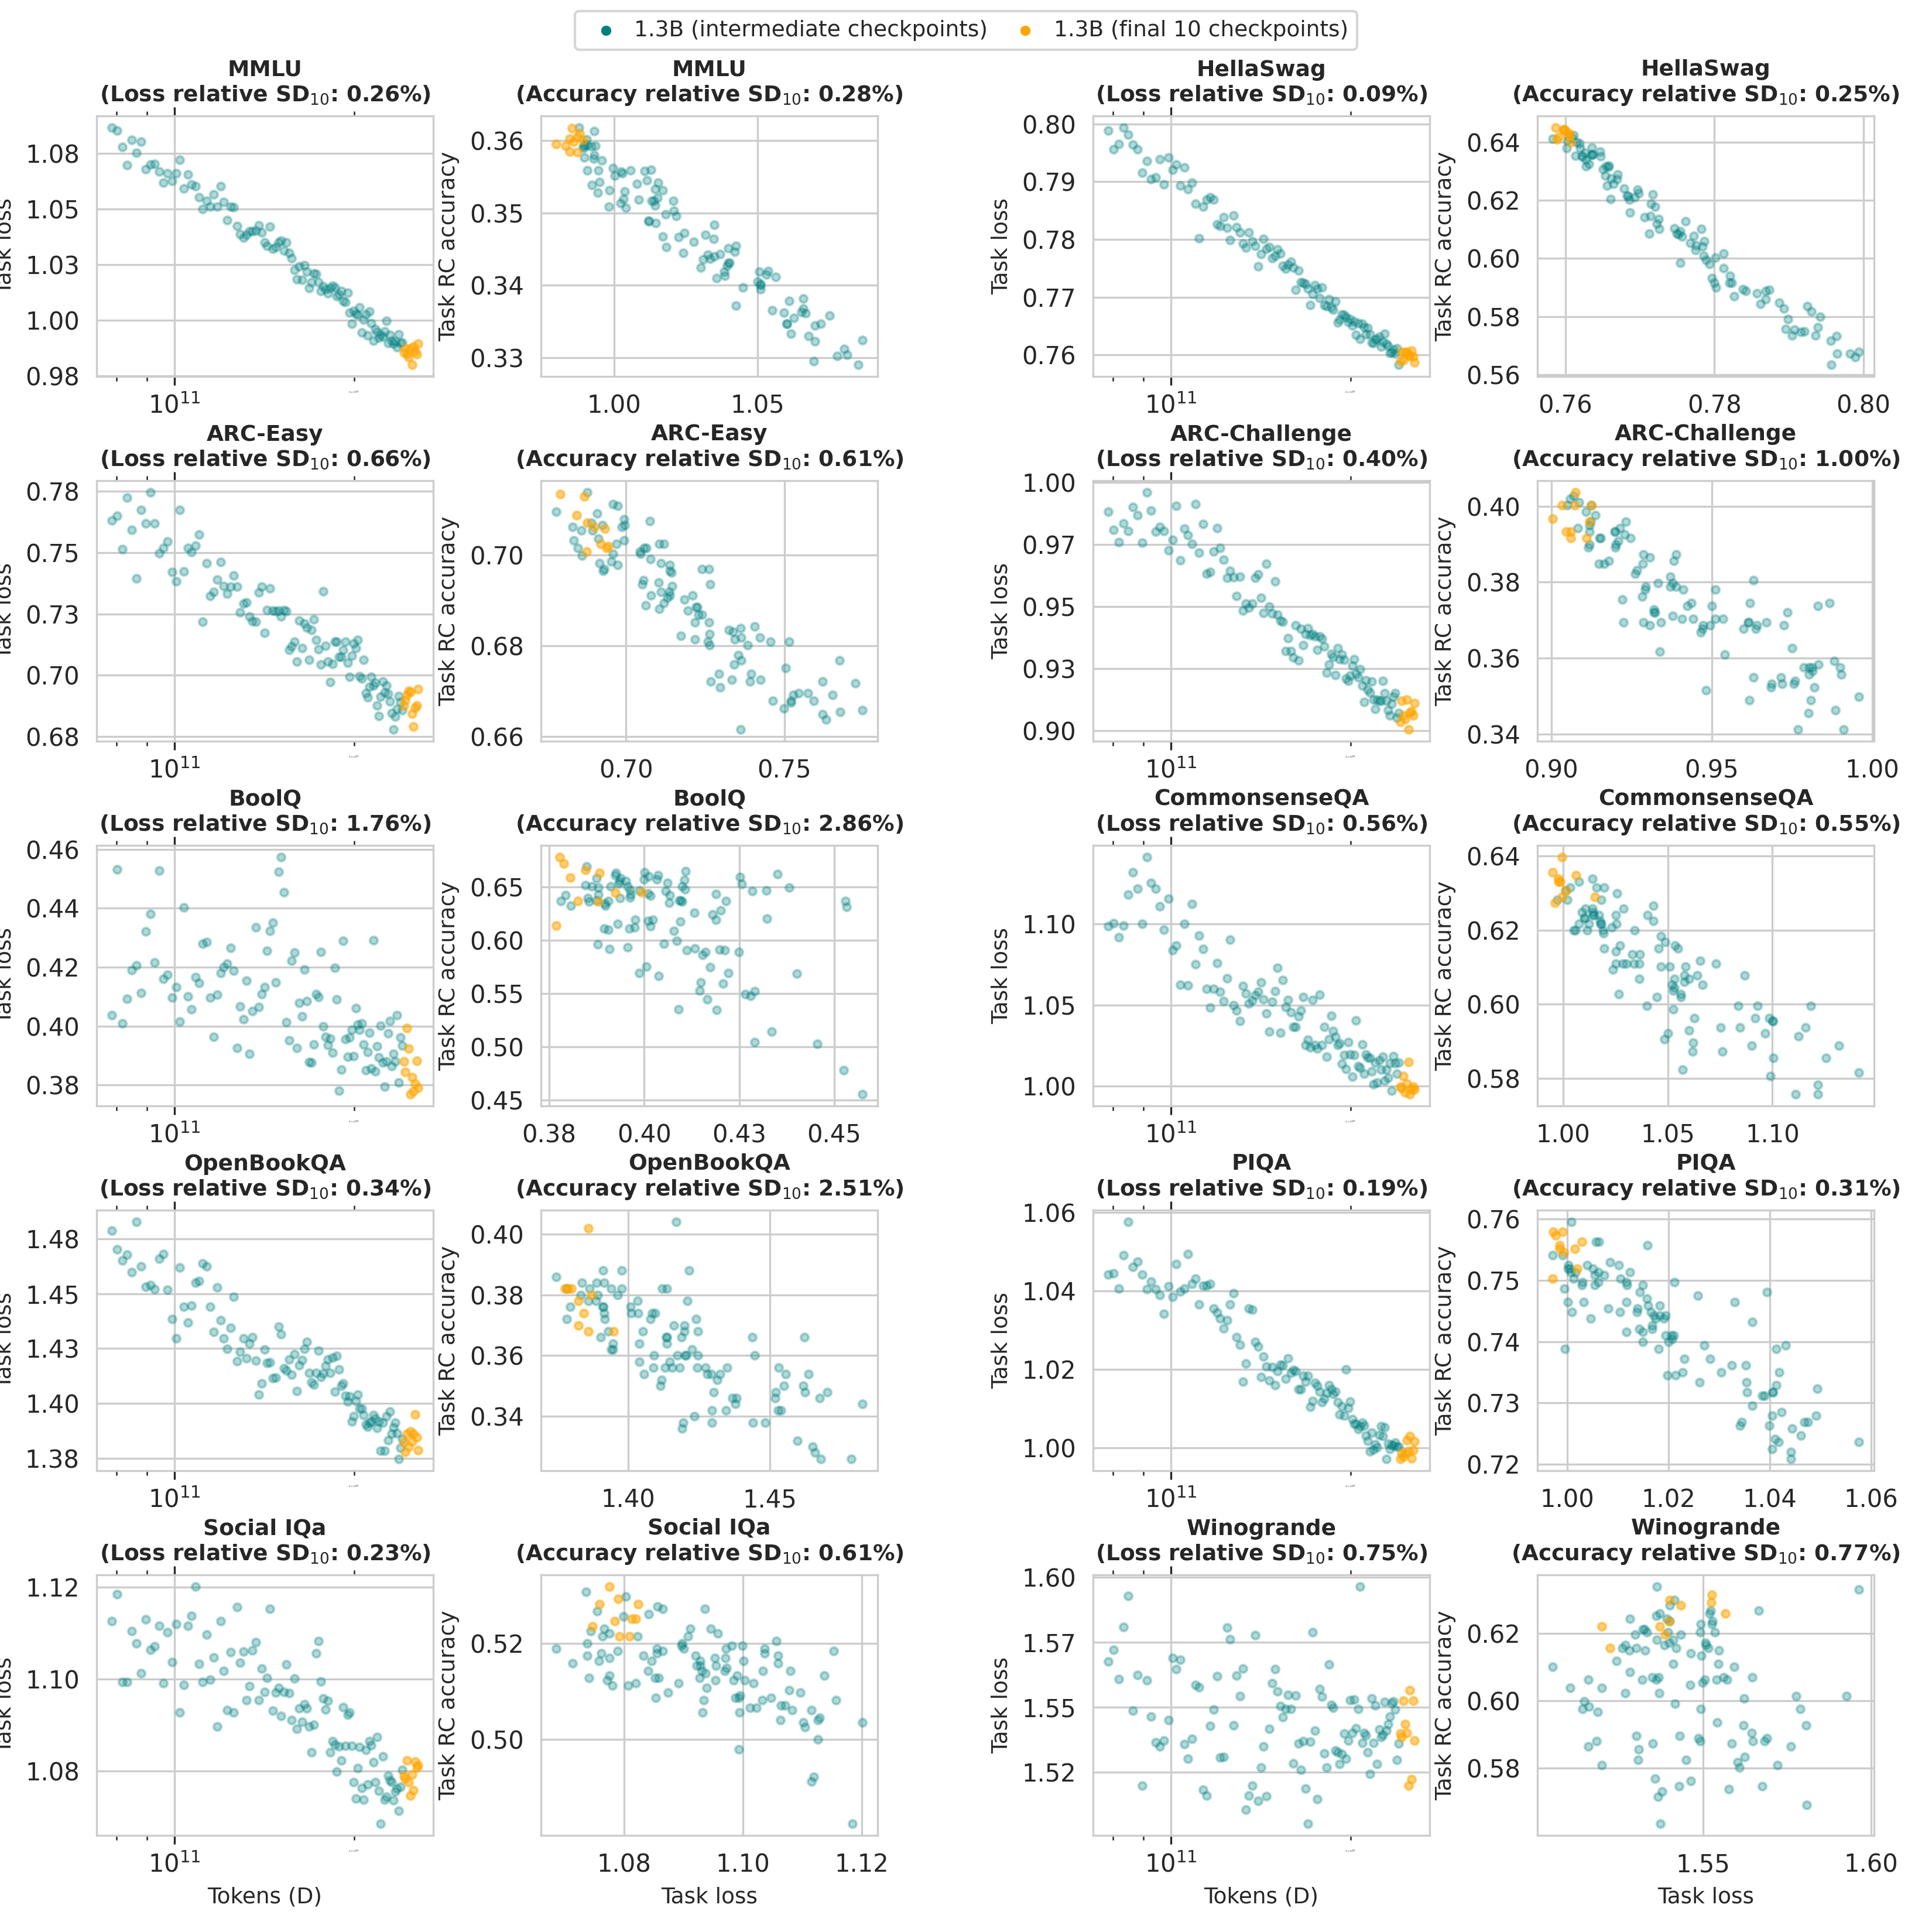
\includegraphics[width=\linewidth]{images/variance_analysis/variance_all.png}
\caption{
Intermediate checkpoints and standard deviation over the final 10 checkpoints (SD$_{10}$) for the 1B-10xC ladder model. 
We find some tasks exhibit high noise between adjacent training checkpoints, which is indicative of the inherent difficulty in predicting performance for such tasks using the model ladder.
}
\label{fig:variance}
\end{figure*}

\subsection{Predicting task accuracy under the MC format}
\label{sec:mc}
In this paper we have been focusing on the ranked classification (RC) format of tasks.
Here, we explore if we can make predictions when problems are written in the multiple-choice (MC) format. This is a challenging problem, as small models often exhibit random performance on standard downstream tasks (e.g., MMLU) until a certain size threshold \citep{Hu2023PredictingEA}. 
Thus, it is not practical to fit the mapping from task loss to MC accuracy in step 2 with data points from the ladder models.
Instead, we use data points from early intermediate checkpoints of the target models.

Observing the MC accuracy curves during training of the 7B-4T and 13B-5T models (\autoref{fig:step2_mc} upper), we find that they have three phases: (1) very early in training, MC accuracy is random; (2) at some point, MC accuracy increases rapidly; (3) finally, it starts growing steadily with more training steps.
The phase of rapid growth for a model is strikingly identical across all tasks: around 70k steps for the 7B-4T model, and around 20k steps for the 13B-5T model.
As a result, the data points $\{(L_i, Acc_i)\}$ fall on a peculiar shape that cannot be described by a sigmoidal function (\autoref{fig:step2_mc} lower left).

Therefore, we fit the sigmoidal curve on data points collected from intermediate checkpoints during the third phase of the MC accuracy curve.
For 7B-4T, we use steps between 170k and 450k; for 13B-5T, we use steps between 50k and 150k.
Noticing that the curves for the two models do not coincide, we fit a function for each model separately (as opposed to a single joint fitting in RC).
We conduct a case study with MMLU and show the fitting and prediction in \autoref{fig:step2_mc} (lower right).
Using data points from the third phase, we can reliably extrapolate the mapping from task loss to MC accuracy.
We predicted the MC accuracy of 7B-4T with 3.0\% relative error, and that of 13B-5T with 1.0\% relative error.
When chaining this with the step 1 fitted function, our end-to-end prediction of MMLU accuracy has an absolute error of 0.3 points on the 7B-4T model, and 0.4 points on the 13B-5T model.

\paragraph{Compute overhead.}
To fit the step 2 function for MC accuracy, we do need to collect data points from an early part of the target model training.
7B-4T is trained for 928k steps, and we use data points up to 450k, which is about 50\% of the full training compute.
13B-5T is trained for 596k steps, and we use data points up to 150k, which is about 25\% of the full training compute.
We note this is significantly more compute than used in the model ladders for predicting RC performance. However, as noted above, smaller models (which are less compute intensive) don't provide useful signal here. This is an opportunity for future work.

\begin{figure*}[t]
\centering
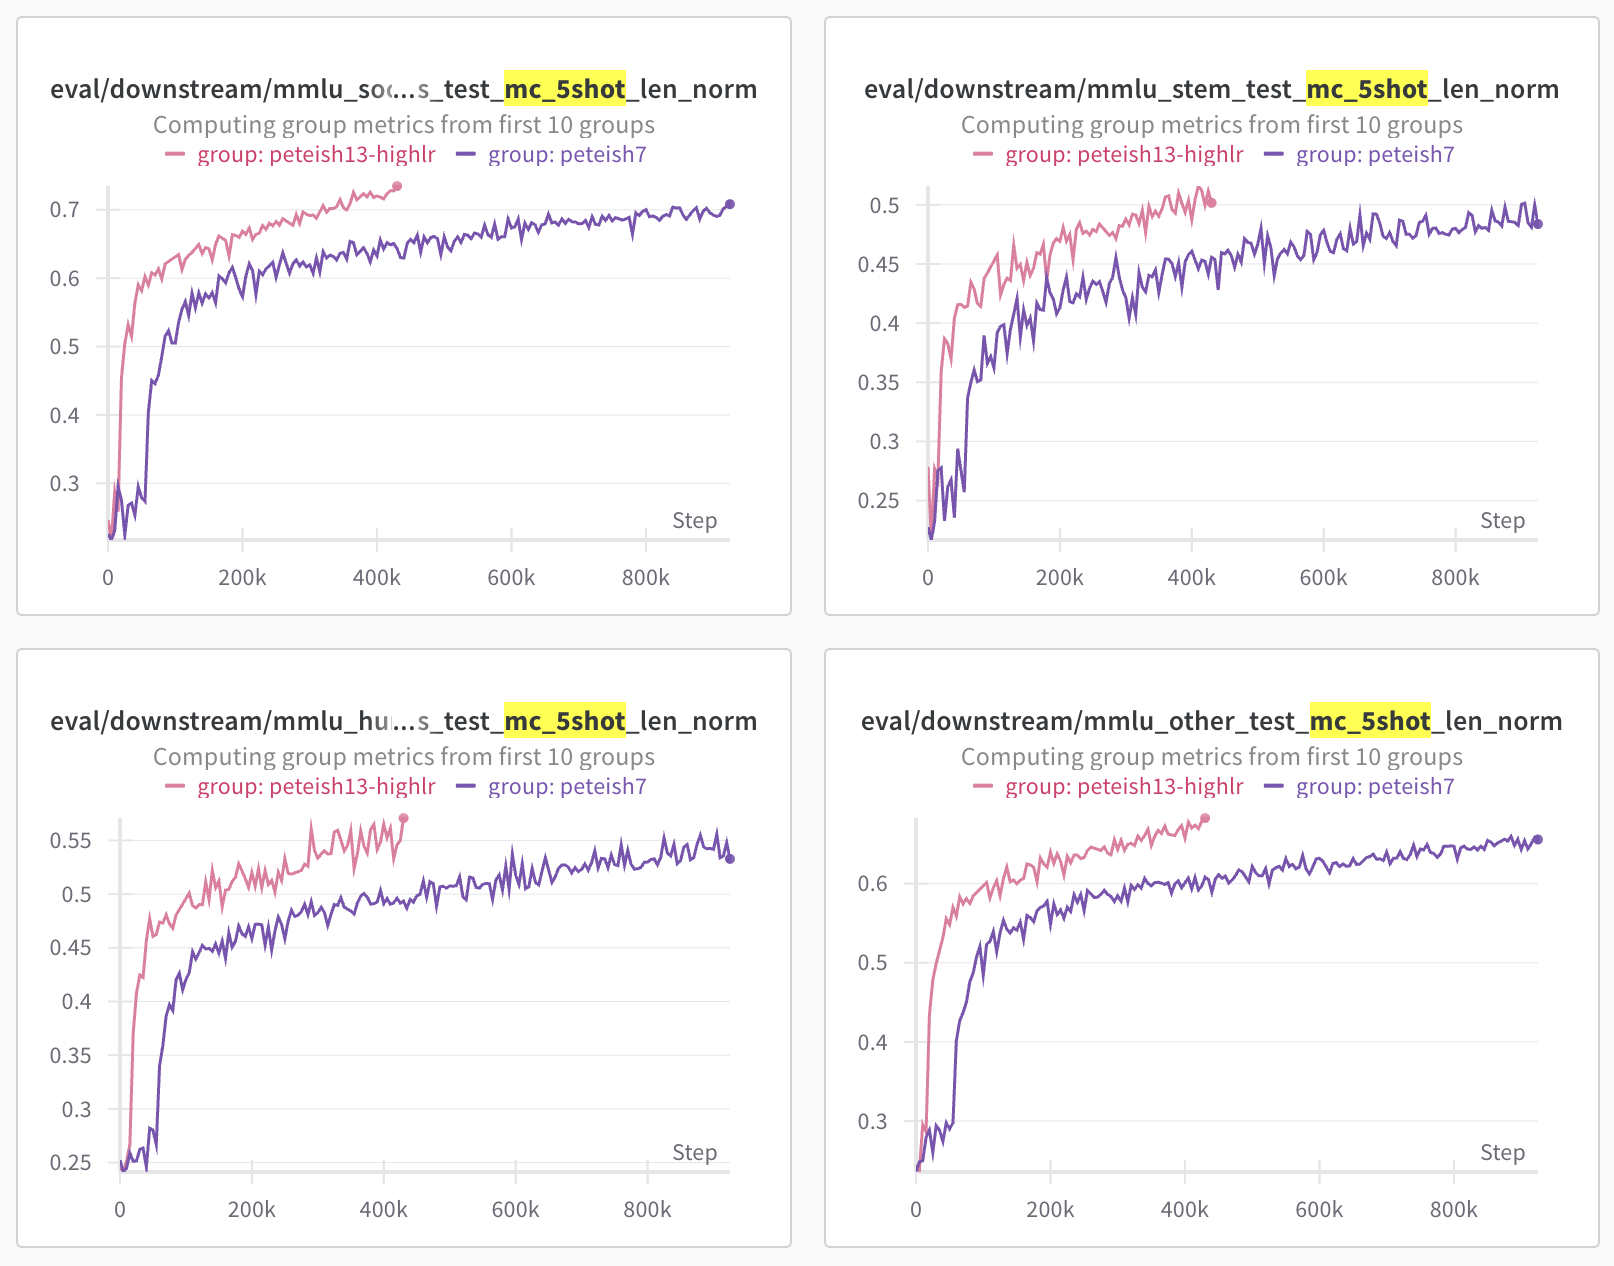
\includegraphics[width=0.39\linewidth]{images/mc_curves_mmlu.png}
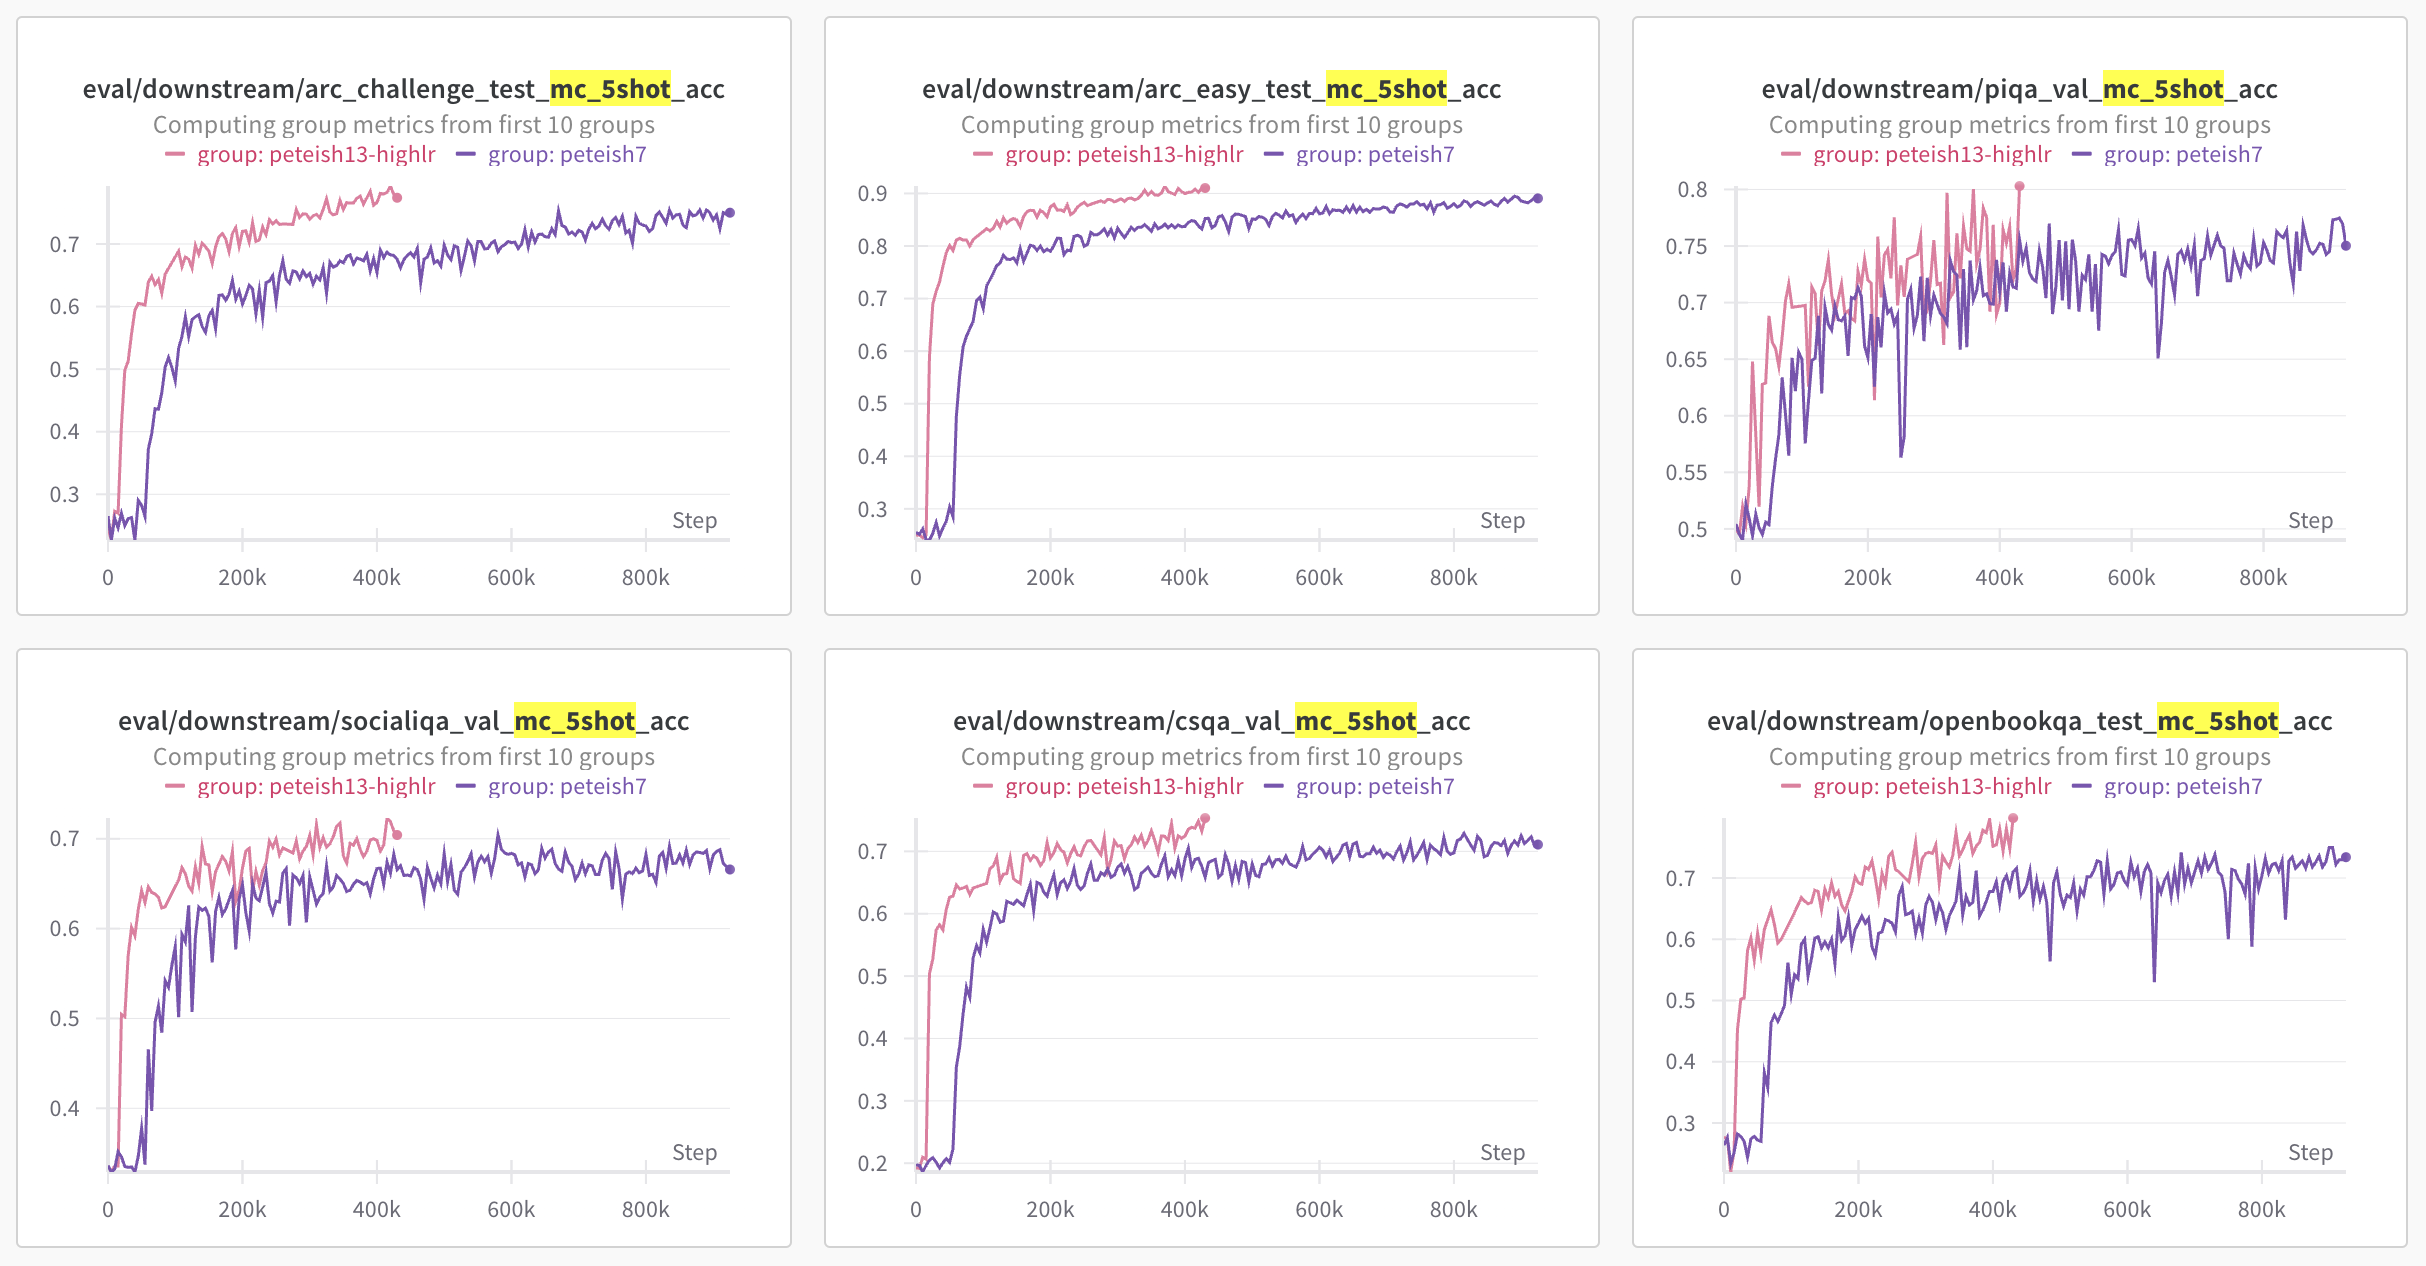
\includegraphics[width=0.59\linewidth]{images/mc_curves_core.png}
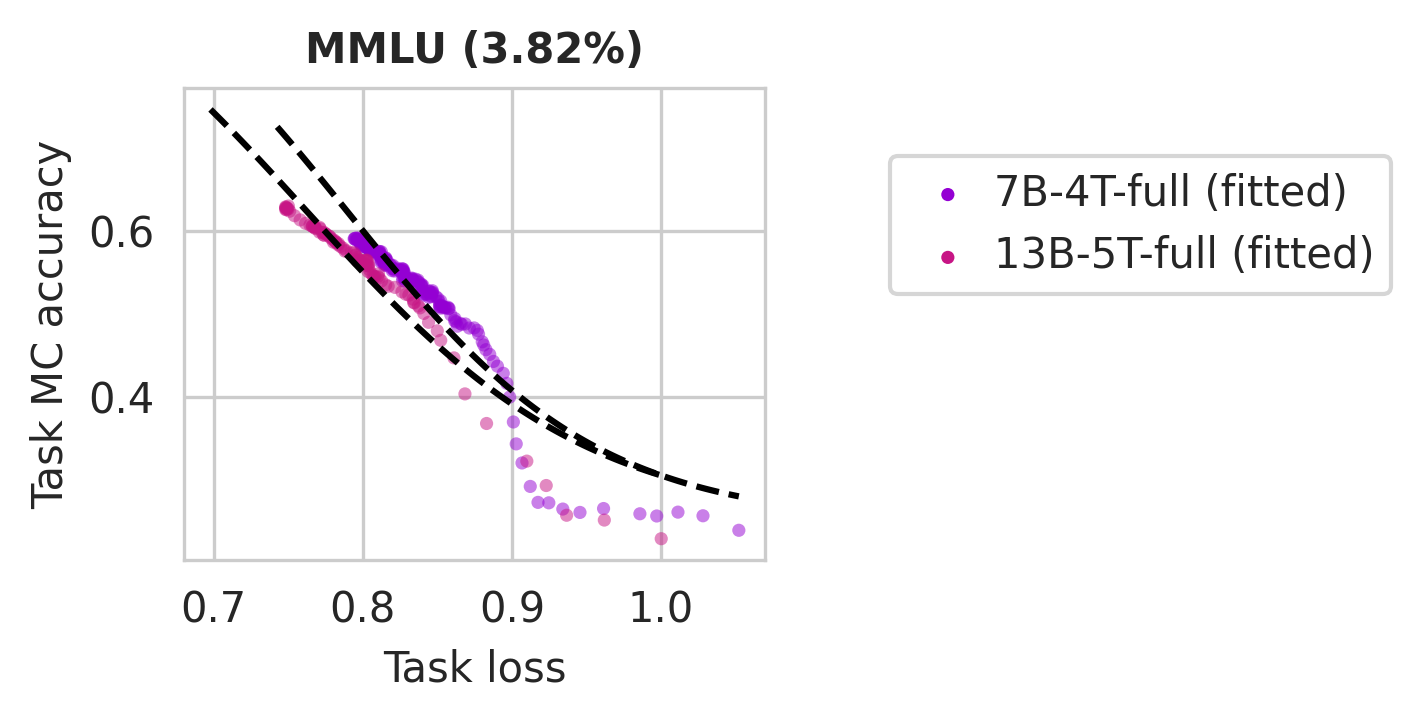
\includegraphics[width=0.49\linewidth]{images/step2_mc_mmlu_full.png}
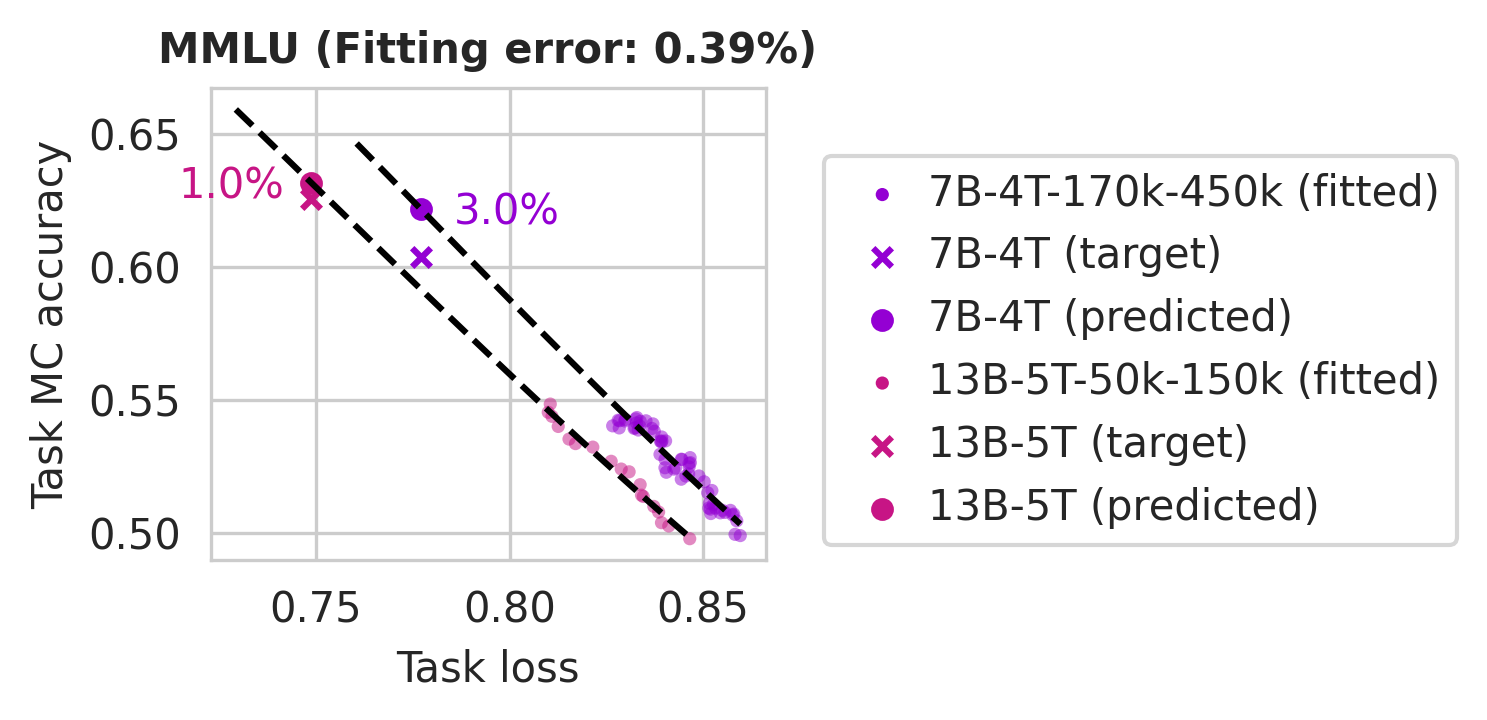
\includegraphics[width=0.49 \linewidth]{images/step2_mc_mmlu.png}
\caption{
    \textbf{Upper:} MC accuracy curves during training of 7B-4T and 13B-5T.
    \textbf{Lower left:} Task MC accuracy vs task loss, with data points from all intermediate checkpoints of 7B-4T and 13B-5T. A sigmoidal function cannot fit the data points.
    \textbf{Lower right:} Task MC accuracy vs task loss, where the sigmoidal function (\autoref{eqn:sigmoid}) is fitted on data points from the intermediate checkpoints between 170k--450k steps of 7B-4T, and between 50k--150k steps of 13B-5T.
}
\label{fig:step2_mc}
% \vspace{-16pt}
\end{figure*}

\begin{figure*}[t]
\centering
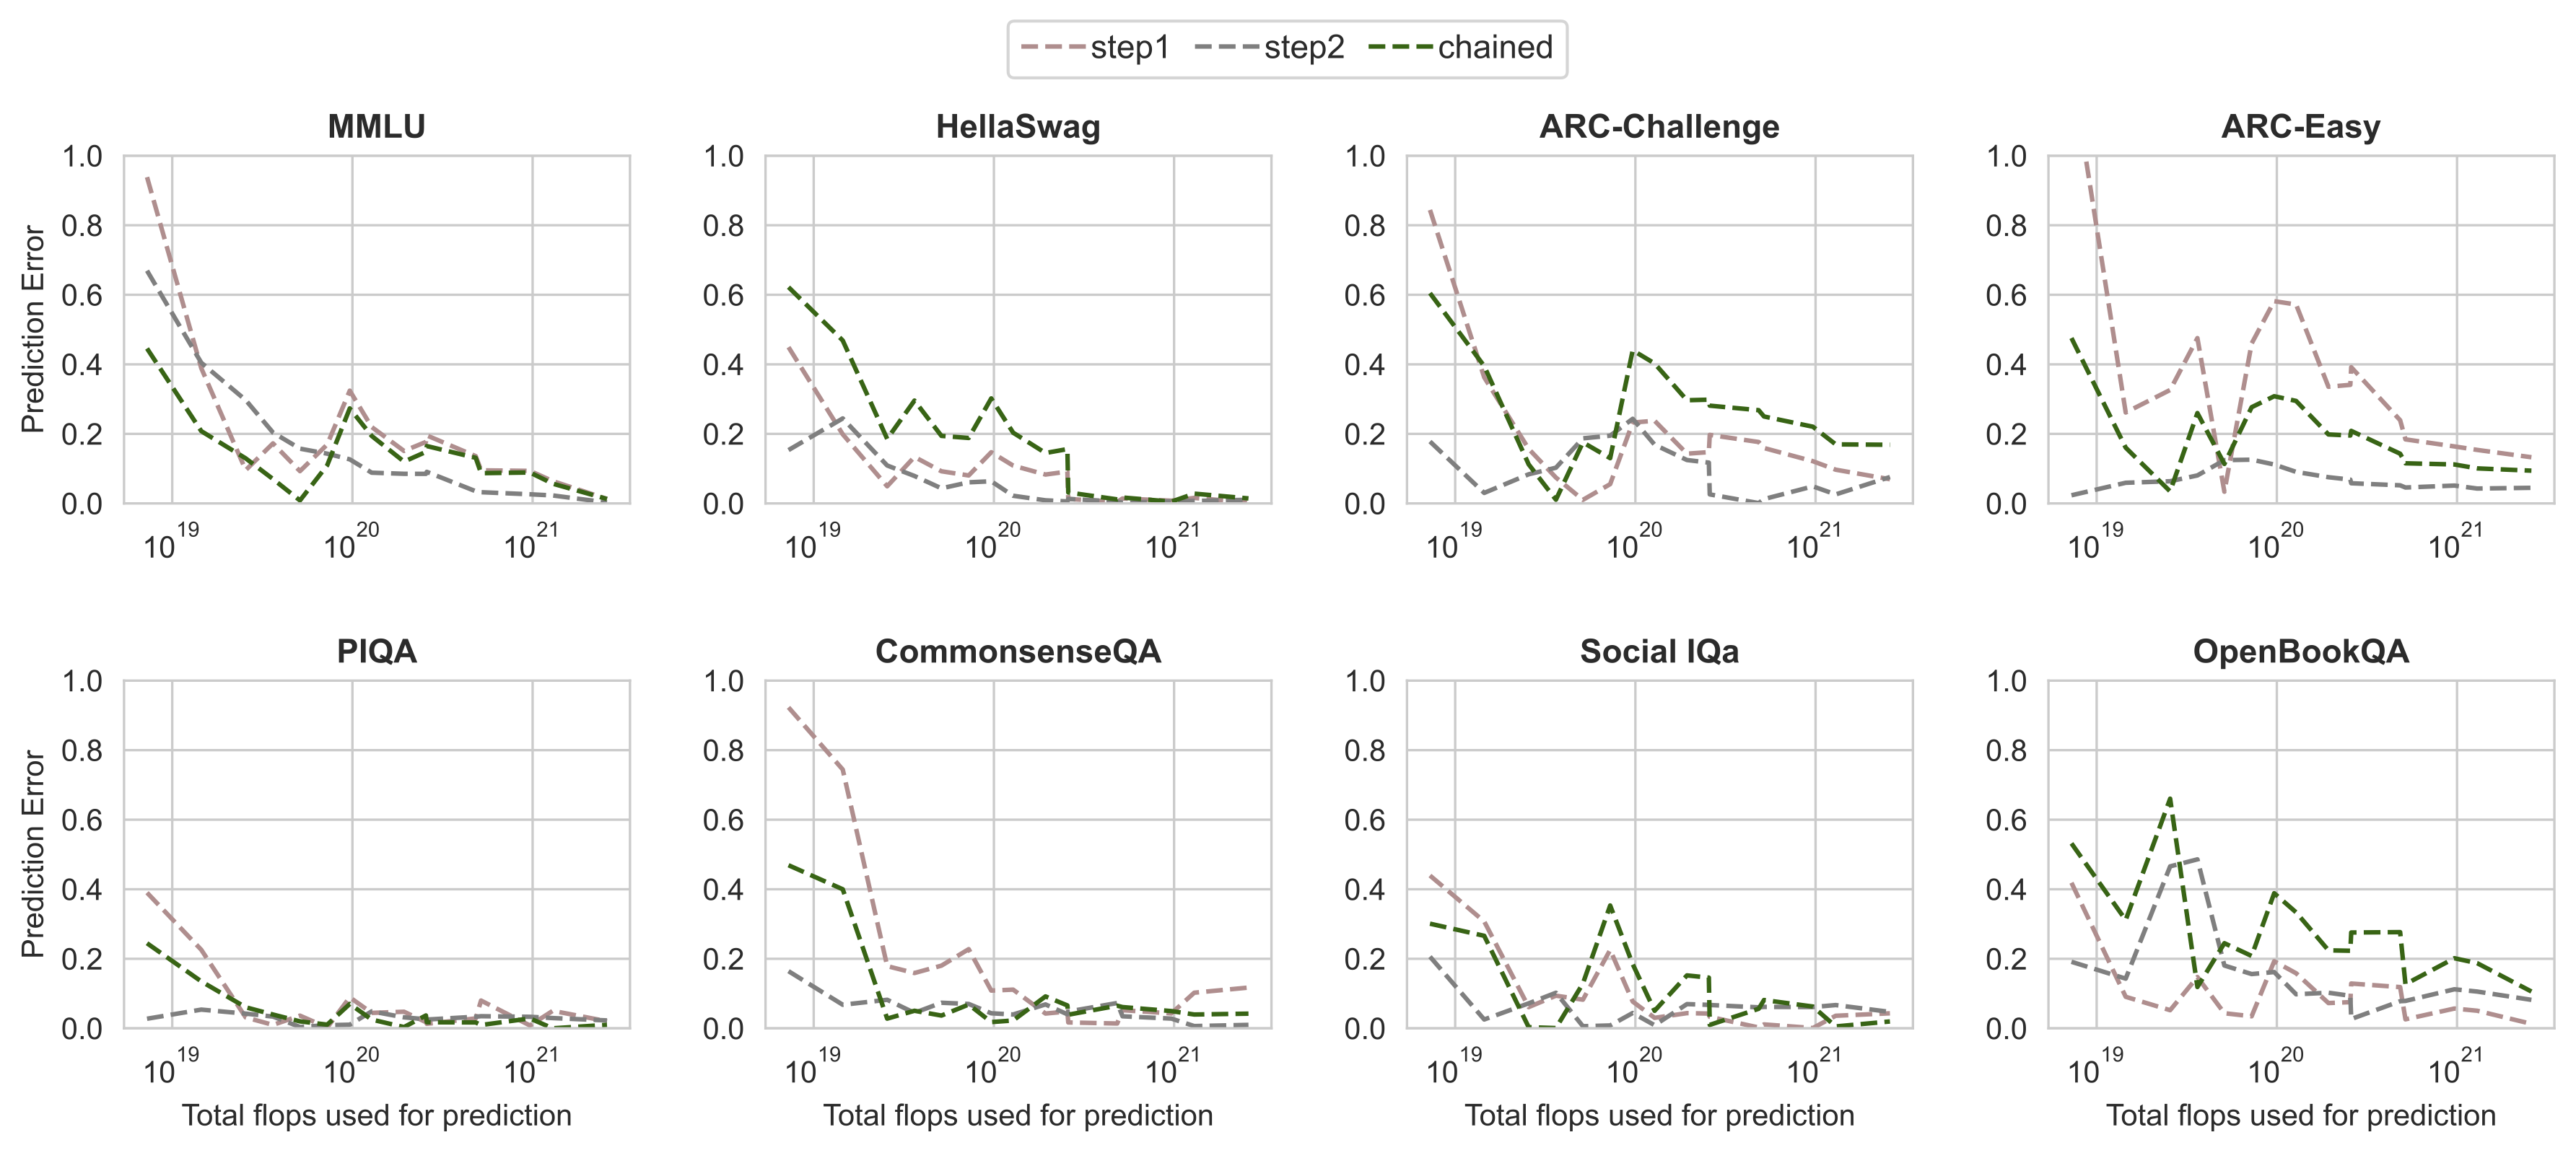
\includegraphics[width=0.8\linewidth]{images/compute_vs_error/vary_flops_error_all.png}
\vspace{-12pt}
\caption{
    Prediction error on the 7B-4T target model as a function of the total compute-FLOPs used in the ladder models for prediction. The left-most point uses only the smallest model (190M-1xC) for prediction. The right-most point uses the full ladder (all 16 models). The prediction error generally reduces as the ladder FLOPs increase. ARC-C, ARC-E, and OBQA display higher variation (which can be attributed to the variation analysis in \S\ref{sec_variance_analysis}), but still have a downward trend.
}
\label{fig:compute_vs_error_flops}
\vspace{-8pt}
\end{figure*}


\subsection{Compute requirements for predicting each task}
\label{app:ablate_compute}

We consider the impact of the scale of the model ladder on the prediction for the target model. In general, the prediction is harder if the difference of scale between the ladder and the target models is larger. We explore this trade-off using the \textbf{7B-4T} model as the target. 

In \autoref{fig:compute_vs_error_flops}, we progressively increase the compute-FLOPs used for function fitting. 
 The prediction error is significantly worse with fewer FLOPs. On MMLU, our full ladder (3.2\% compute of the target model) gets 1.3\% error. Reducing the number of FLOPs to 0.1\% of the target model compute increases the error to $\sim$12\% which is an order of magnitude higher. This is more observable in certain tasks. Interestingly, we see a slight improvement in errors with less compute in ARC-C and ARC-E, potentially due to the variance as seen in \S\ref{sec_variance_analysis}.

We also consider the impact of each axis of the ladder models (model size $N$ and Chinchilla multiplier $xC$) on the prediction error for each task. 

\autoref{fig:compute_vs_error_N} shows the prediction errors for each step as we progressively increase the model size included in the ladder (i.e., ladder upto 760M will include 190M, 370M, 760M). We observe a downward trend in the prediction error for most tasks as the ladder size gets closer to the target model. 

\begin{figure*}[t]
\centering
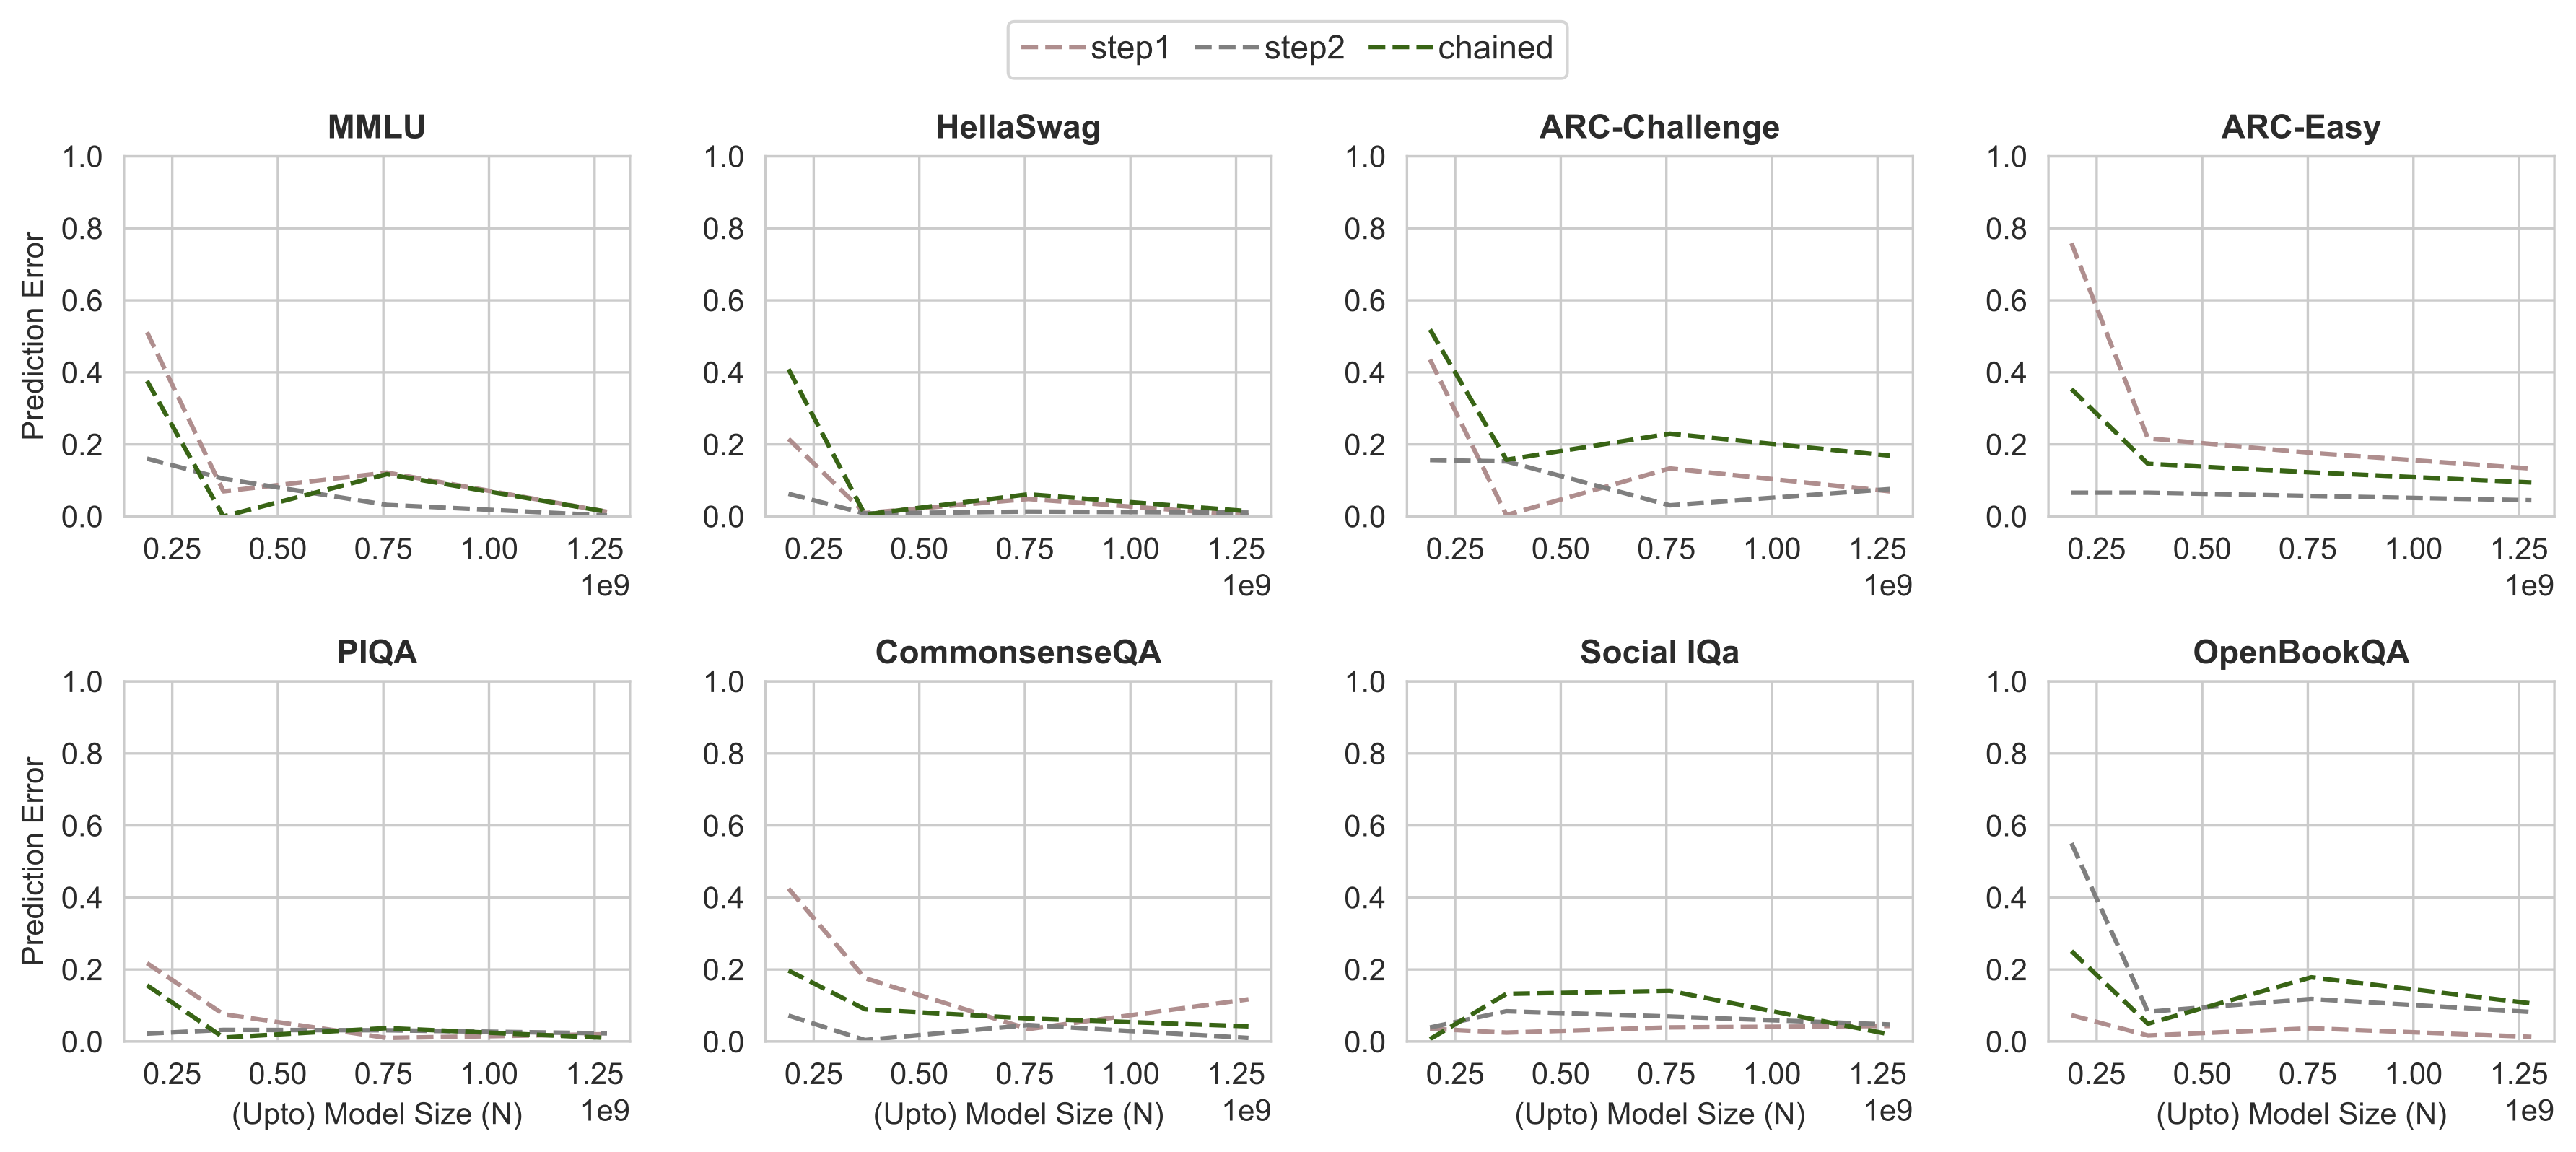
\includegraphics[width=0.90\linewidth]{images/compute_vs_error/vary_N_error_all.png}
\vspace{-12pt}
\caption{
    Prediction error on the 7B-4T target model when including \textbf{up to} model size ($N$) in the ladder for prediction. Eg. $N$ up to 760M will include 190M, 370M, 760M models trained to 1xC, 2xC, 5xC, 10xC. For most tasks, we observe a downward trend in the prediction error as $N$ increases.
}
\label{fig:compute_vs_error_N}
\vspace{-8pt}
\end{figure*}

\autoref{fig:compute_vs_error_xC} similarly shows the impact of including models with longer training regimes. Interestingly, we do not see a significant reduction in the prediction error as we include the ladder models trained to higher Chinchilla multipliers\footnote{The target model 7B-4T is trained to approximately 28xC.}. There is a slight downward trend (noticeable in MMLU), but this dimension has more flexibility. 

For users of our approach, and future work, we encourage exploration in reducing the overall cost by considering both these dimensions. Concretely, given a fixed budget for the ladder models, increasing the model size $N$ is more likely to improve the prediction error, compared to training for longer.

\begin{figure*}[t]
\centering
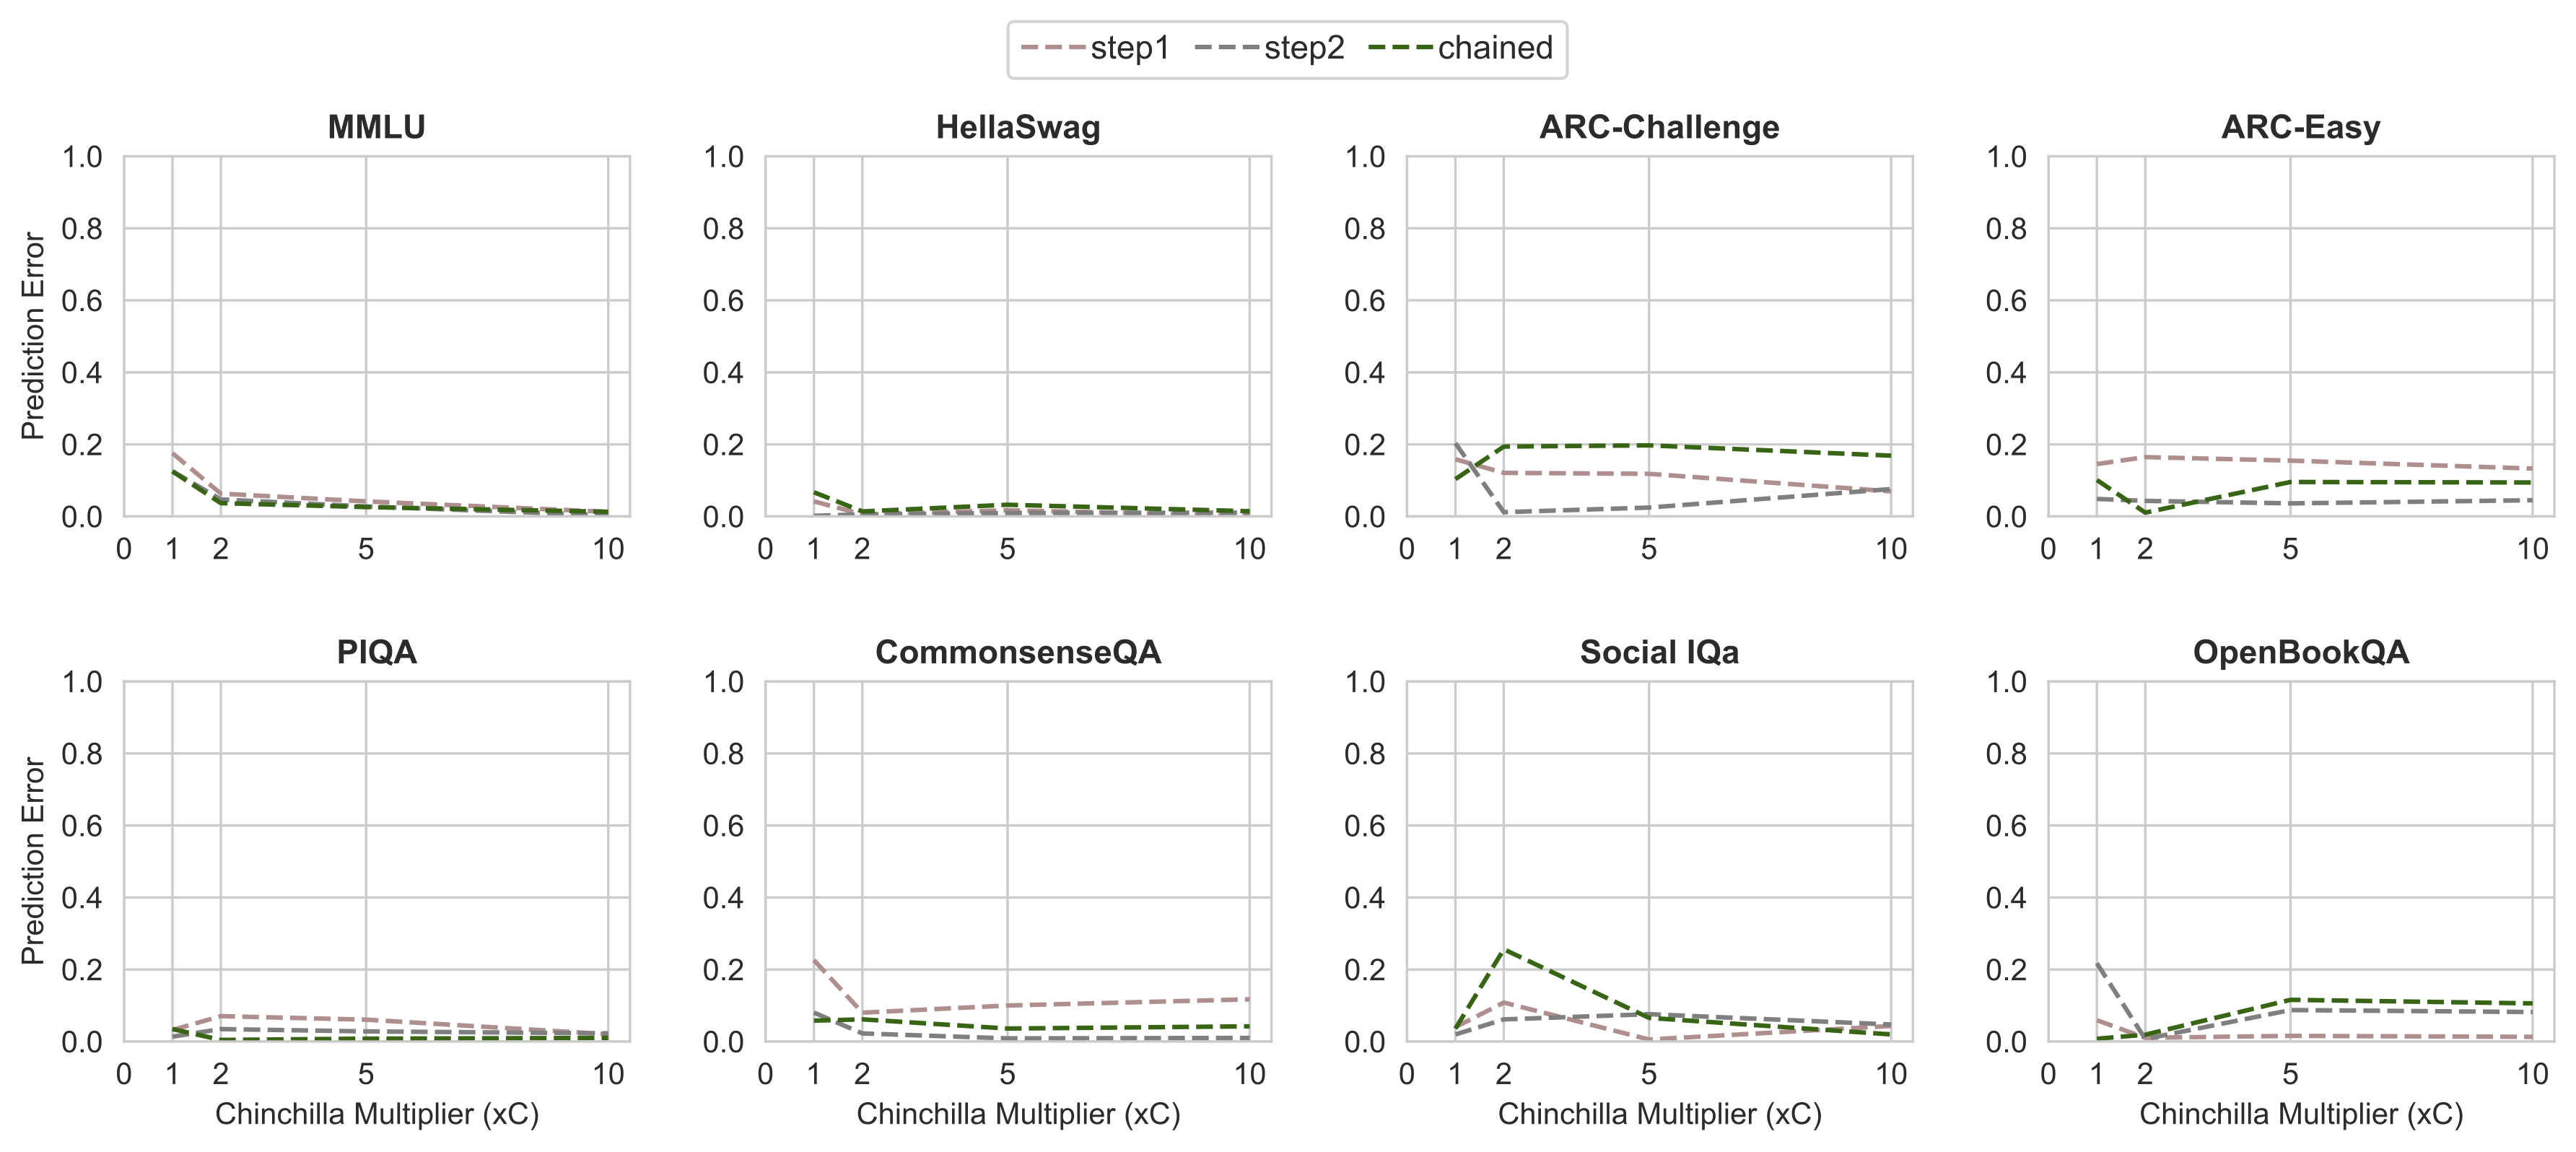
\includegraphics[width=0.90\linewidth]{images/compute_vs_error/vary_xC_error_all.png}
\vspace{-12pt}
\caption{
    Prediction error on the 7B-4T target model when including models trained \textbf{up to} chinchilla multiplier ($xC$). Eg. $xC$ up to 2xC will include 190M, 370M, 760M, 1B models trained to 1xC, 2xC. The downward trend of the prediction error is less significant than with varying $N$. 
}
\label{fig:compute_vs_error_xC}
\vspace{-8pt}
\end{figure*}

\section{Additional Details on Design Choices}
\label{app:ablations}

\subsection{Compute-FLOPs $C$ instead of $(N, D)$ for task loss prediction}
\label{app:flops_as_feature}

We test if compute-FLOPs $C$ can be used directly for task loss prediction instead of $(N, D)$ in the over-trained regime with the ladder models.
We fit a similar power function
\begin{align}
L(C) &= A / C^\alpha + E
\label{eqn:flops_fit}
\end{align}
where $A, \alpha, E$ are parameters to fit.

\begin{figure*}[h!]
\centering
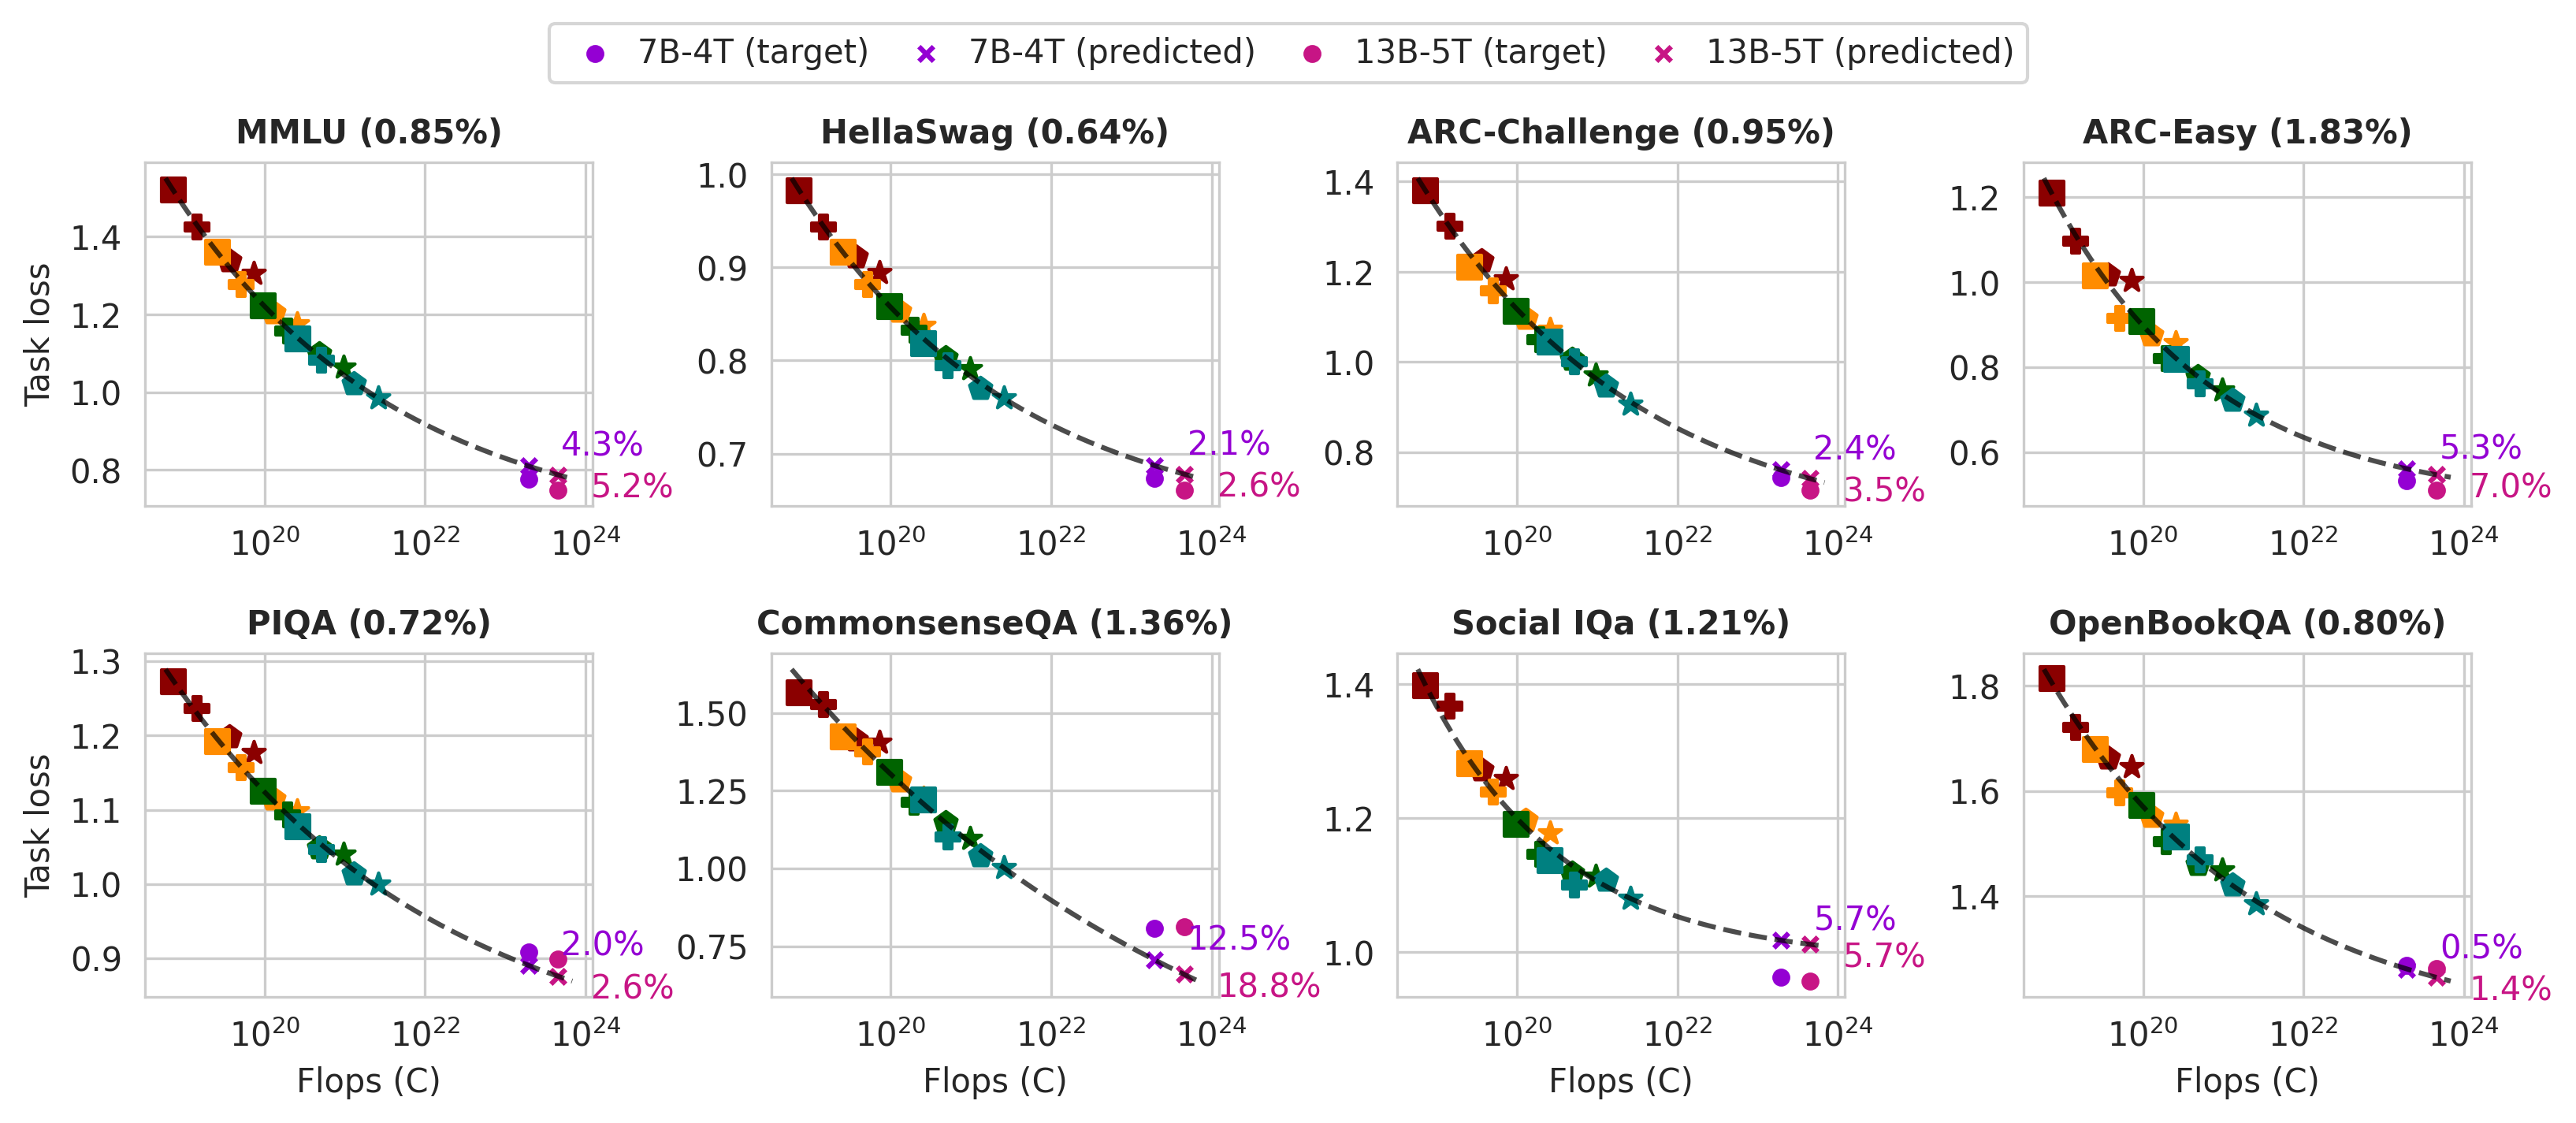
\includegraphics[width=1.0 \linewidth]{images/step1_flops_main.png}
\caption{
    Step 1 using compute-flops $C$ instead of $(N, D)$.
    \ding{110} = 1xC; \ding{58} = 2xC; $\pentagofill$ = 5xC; $\bigstar$ = 10xC.
    We report the average relative fitting error in parentheses following the task name, and prediction error in the plot next to the target model point.
}
\label{fig:step1_flops}
% \vspace{-16pt}
\end{figure*}

\autoref{fig:step1_flops} shows the function fitting and prediction.
Compared with \autoref{fig:step1}, the relative fitting error is higher than using $(N, D)$ on all tasks, likely because \autoref{eqn:flops_fit} has fewer free parameters than \autoref{eqn:power}.
For the target models, the task loss prediction errors are generally worse than using $(N, D)$, including on MMLU; ARC-Challenge and ARC-Easy are the outliers (\autoref{tab:design_choices}).

Overall, compute-FLOPs are not expressive enough to distinguish between compute-optimal and overtrained models with equal FLOPs but different losses \citep{Hoffmann2022TrainingCL}.
Thus, we do not use it in our main method.

% \autoref{fig:step1_flops} shows the function fitting and prediction in step 1, using compute-FLOPs as the input feature.

\subsection{Task cross-entropy as the intermediate feature}
\label{app:task_ce}

Task loss only considers the correct choice of each problem. However, task RC accuracy is determined by the losses of both correct and incorrect choices, which is a major challenge for predicting downstream performance \citep{schaeffer2024why}:

\begin{equation} \label{eqn:task_acc}
\text{Acc} = \frac{1}{N} \sum_{i=1}^N \mathbbm{1} \left[ \arg\max_{k} \left( {-L_k^{(i)}} \right) = \hat k^{(i)} \right],
\end{equation}
where $L_k^{(i)}$ is the loss over the $k$'th answer option of the $i$'th example and $\hat k^{(i)}$ is the label of the correct answer \footnote{Loss terms may include some normalization, e.g., by the number of characters in each answer or the unconditional answer probability \citep{gu2024olmes}.}. 

To account for incorrect answers, we define an alternative intermediate feature. We commonly maximize the accuracy by minimizing the task cross-entropy as a surrogate loss, in which the $L_k$ terms are used as logits:
\begin{equation} \label{eqn:task_ce}
\text{TaskCE} = \frac{1}{N} \sum_{i=1}^N \left( {L^{(i)}_{\hat k^{(i)}}} + \log {\sum_k \exp \left( -L^{(i)}_{k} \right) } \right).
\end{equation}
We refer to this as TaskCE to distinguish it from the language modeling cross-entropy over tokens.

\begin{table*}[t]
\small
\setlength{\tabcolsep}{3pt}
\centering
\begin{tabular}{l | r r r r | r r r r}
\toprule
 & \multicolumn{4}{c|}{\textbf{7B-4T}} & \multicolumn{4}{c}{\textbf{13B-5T}} \\
& \multicolumn{2}{c}{BPB} & \multicolumn{2}{c|}{TaskCE} & \multicolumn{2}{c}{BPB} & \multicolumn{2}{c}{TaskCE} \\
& Error &  \%Error & Error &  \%Error & Error &  \%Error & Error &  \%Error  \\
\midrule
MMLU & 0.6 & 1.3\% & 9.0 & 18.3\% & 0.3 & 0.6\% & 10.4 & 20.2\% \\
HellaSwag & 1.2 & 1.4\% & 5.9 & 7.2\% & 2.1 & 2.5\% & 8.7 & 10.5\% \\
ARC-Challenge & 10.4 & 16.9\% & 13.1 & 21.3\% & 11.1 & 17.5\% & 12.3 & 19.5\% \\
ARC-Easy & 8.0 & 9.4\% & 4.5 & 5.4\% & 10.0 & 11.4\% & 5.4 & 6.2\% \\
PIQA & 0.8 & 1.0\% & 2.5 & 3.1\% & 0.9 & 1.1\% & 2.4 & 2.9\% \\
CommonsenseQA & 3.1 & 4.2\% & 1.9 & 2.6\% & 3.5 & 4.7\% & 2.0 & 2.7\% \\
Social IQa & 1.2 & 2.0\% & 0.5 & 0.7\% & 1.7 & 2.7\% & 0.8 & 1.2\% \\
OpenBookQA & 5.2 & 10.6\% & 3.5 & 7.1\% & 3.7 & 7.8\% & 0.1 & 0.2\% \\
\bottomrule
\end{tabular}
\caption{
    Comparison of original and new prediction errors for 7B-4T and 13B-5T models across tasks. Absolute (Error) and relative (\%Error) differences are shown.
}
\label{tab:updated_pred_taskce}
\end{table*}


\begin{figure*}[ht]
    \centering
    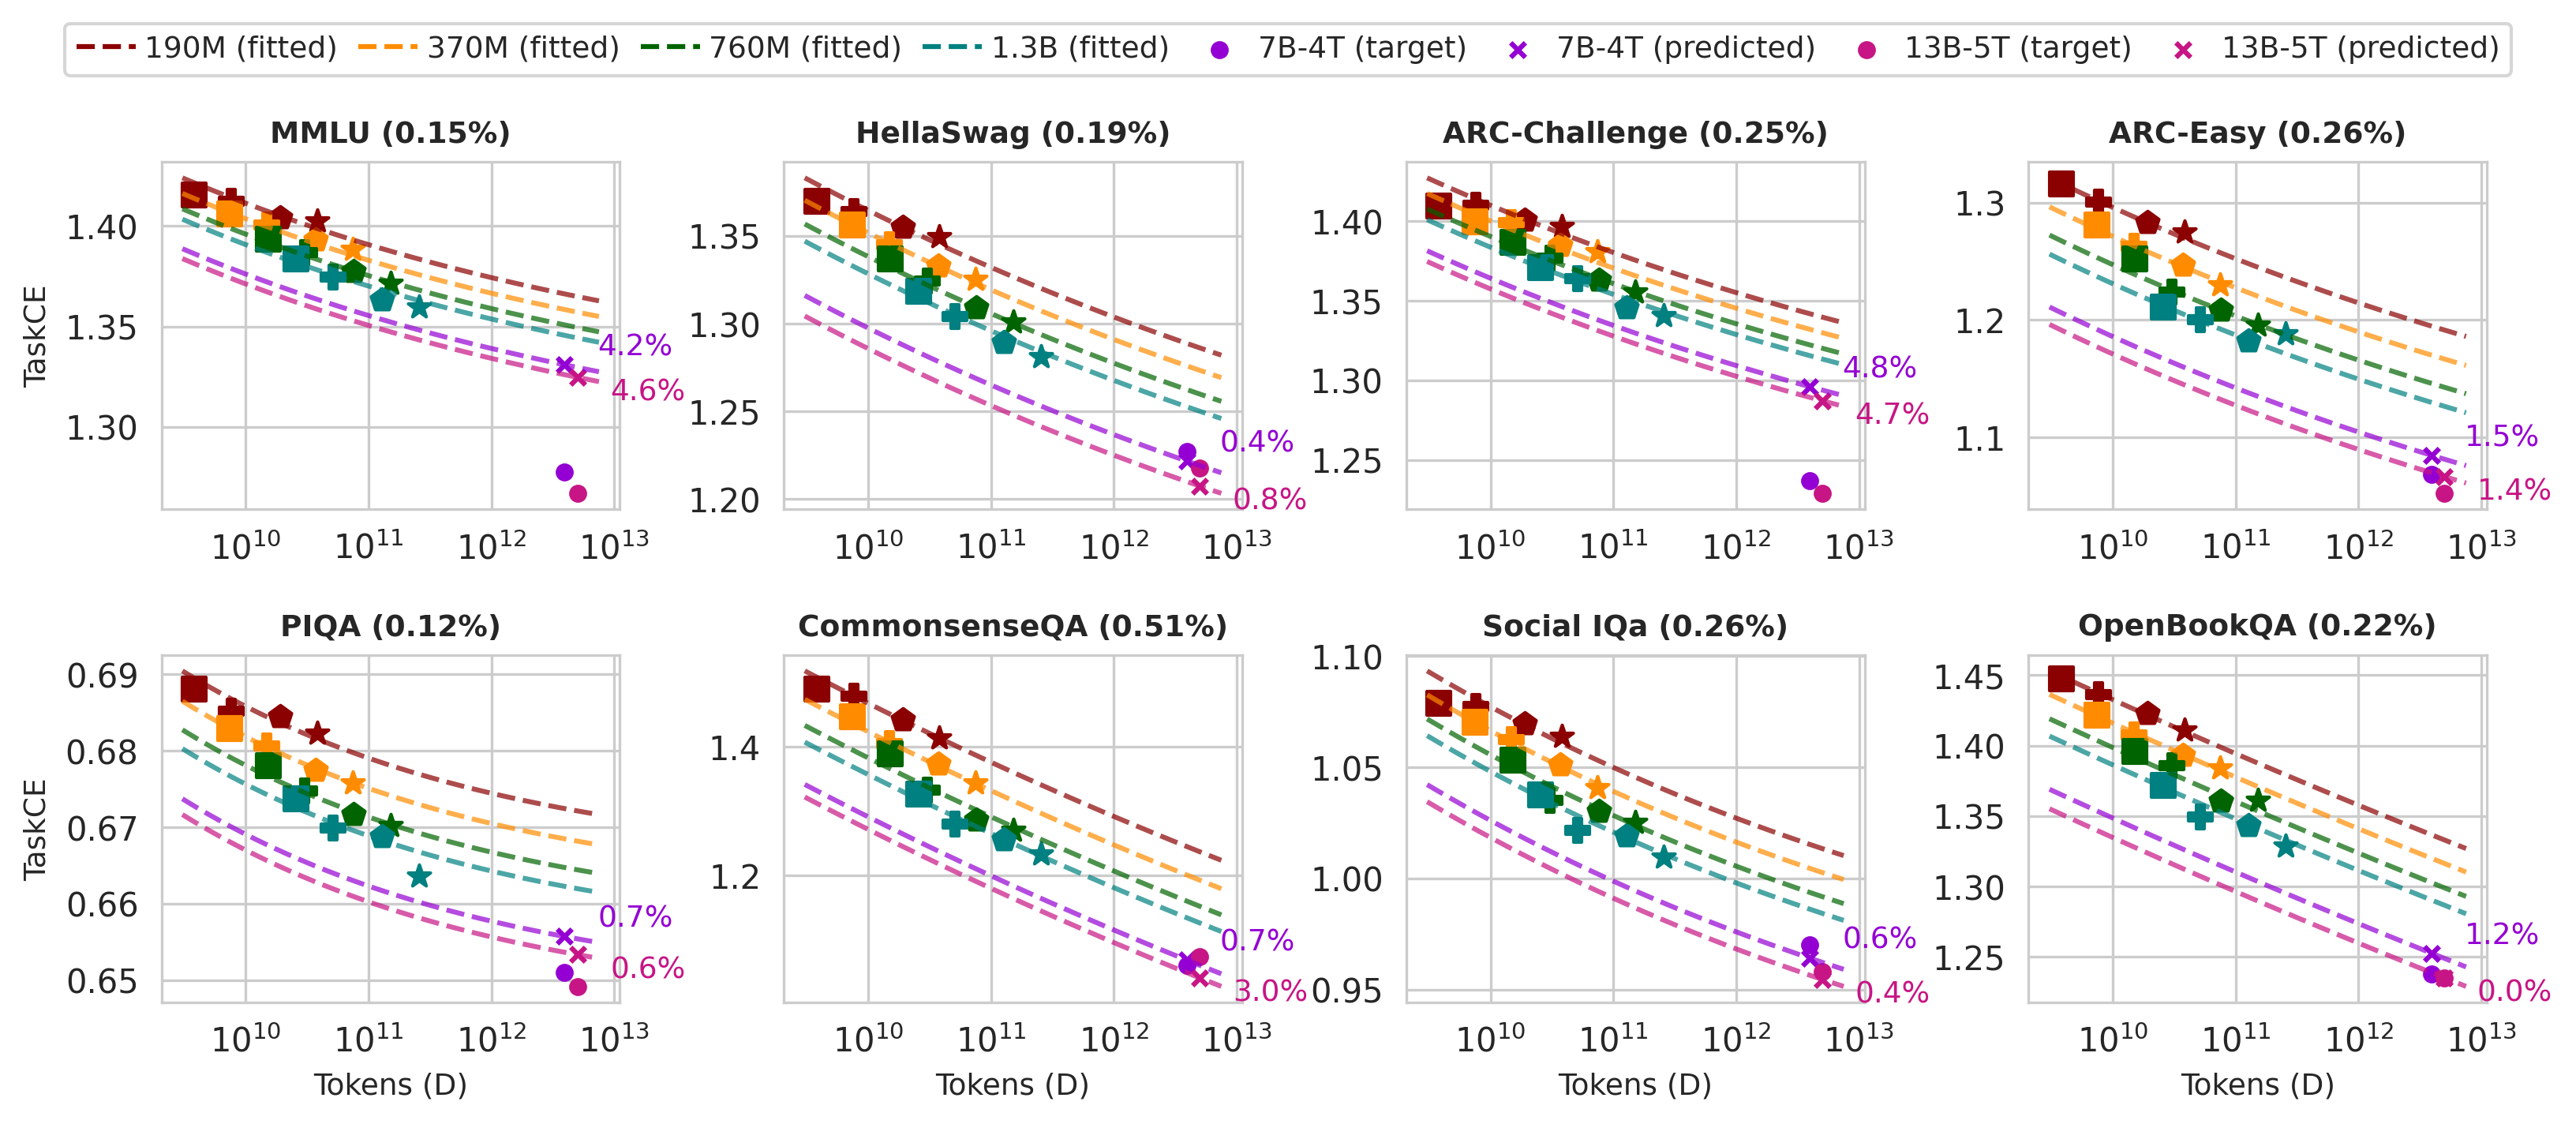
\includegraphics[width=\linewidth]{images/step1_taskce_main.png}
    \caption{Predicting final \textit{task cross-entropy} (\autoref{eqn:task_ce}) from model parameters and token budget in step 1.}
    \label{fig:step1_taskce}
\end{figure*}


\begin{figure*}[ht]
    \centering
    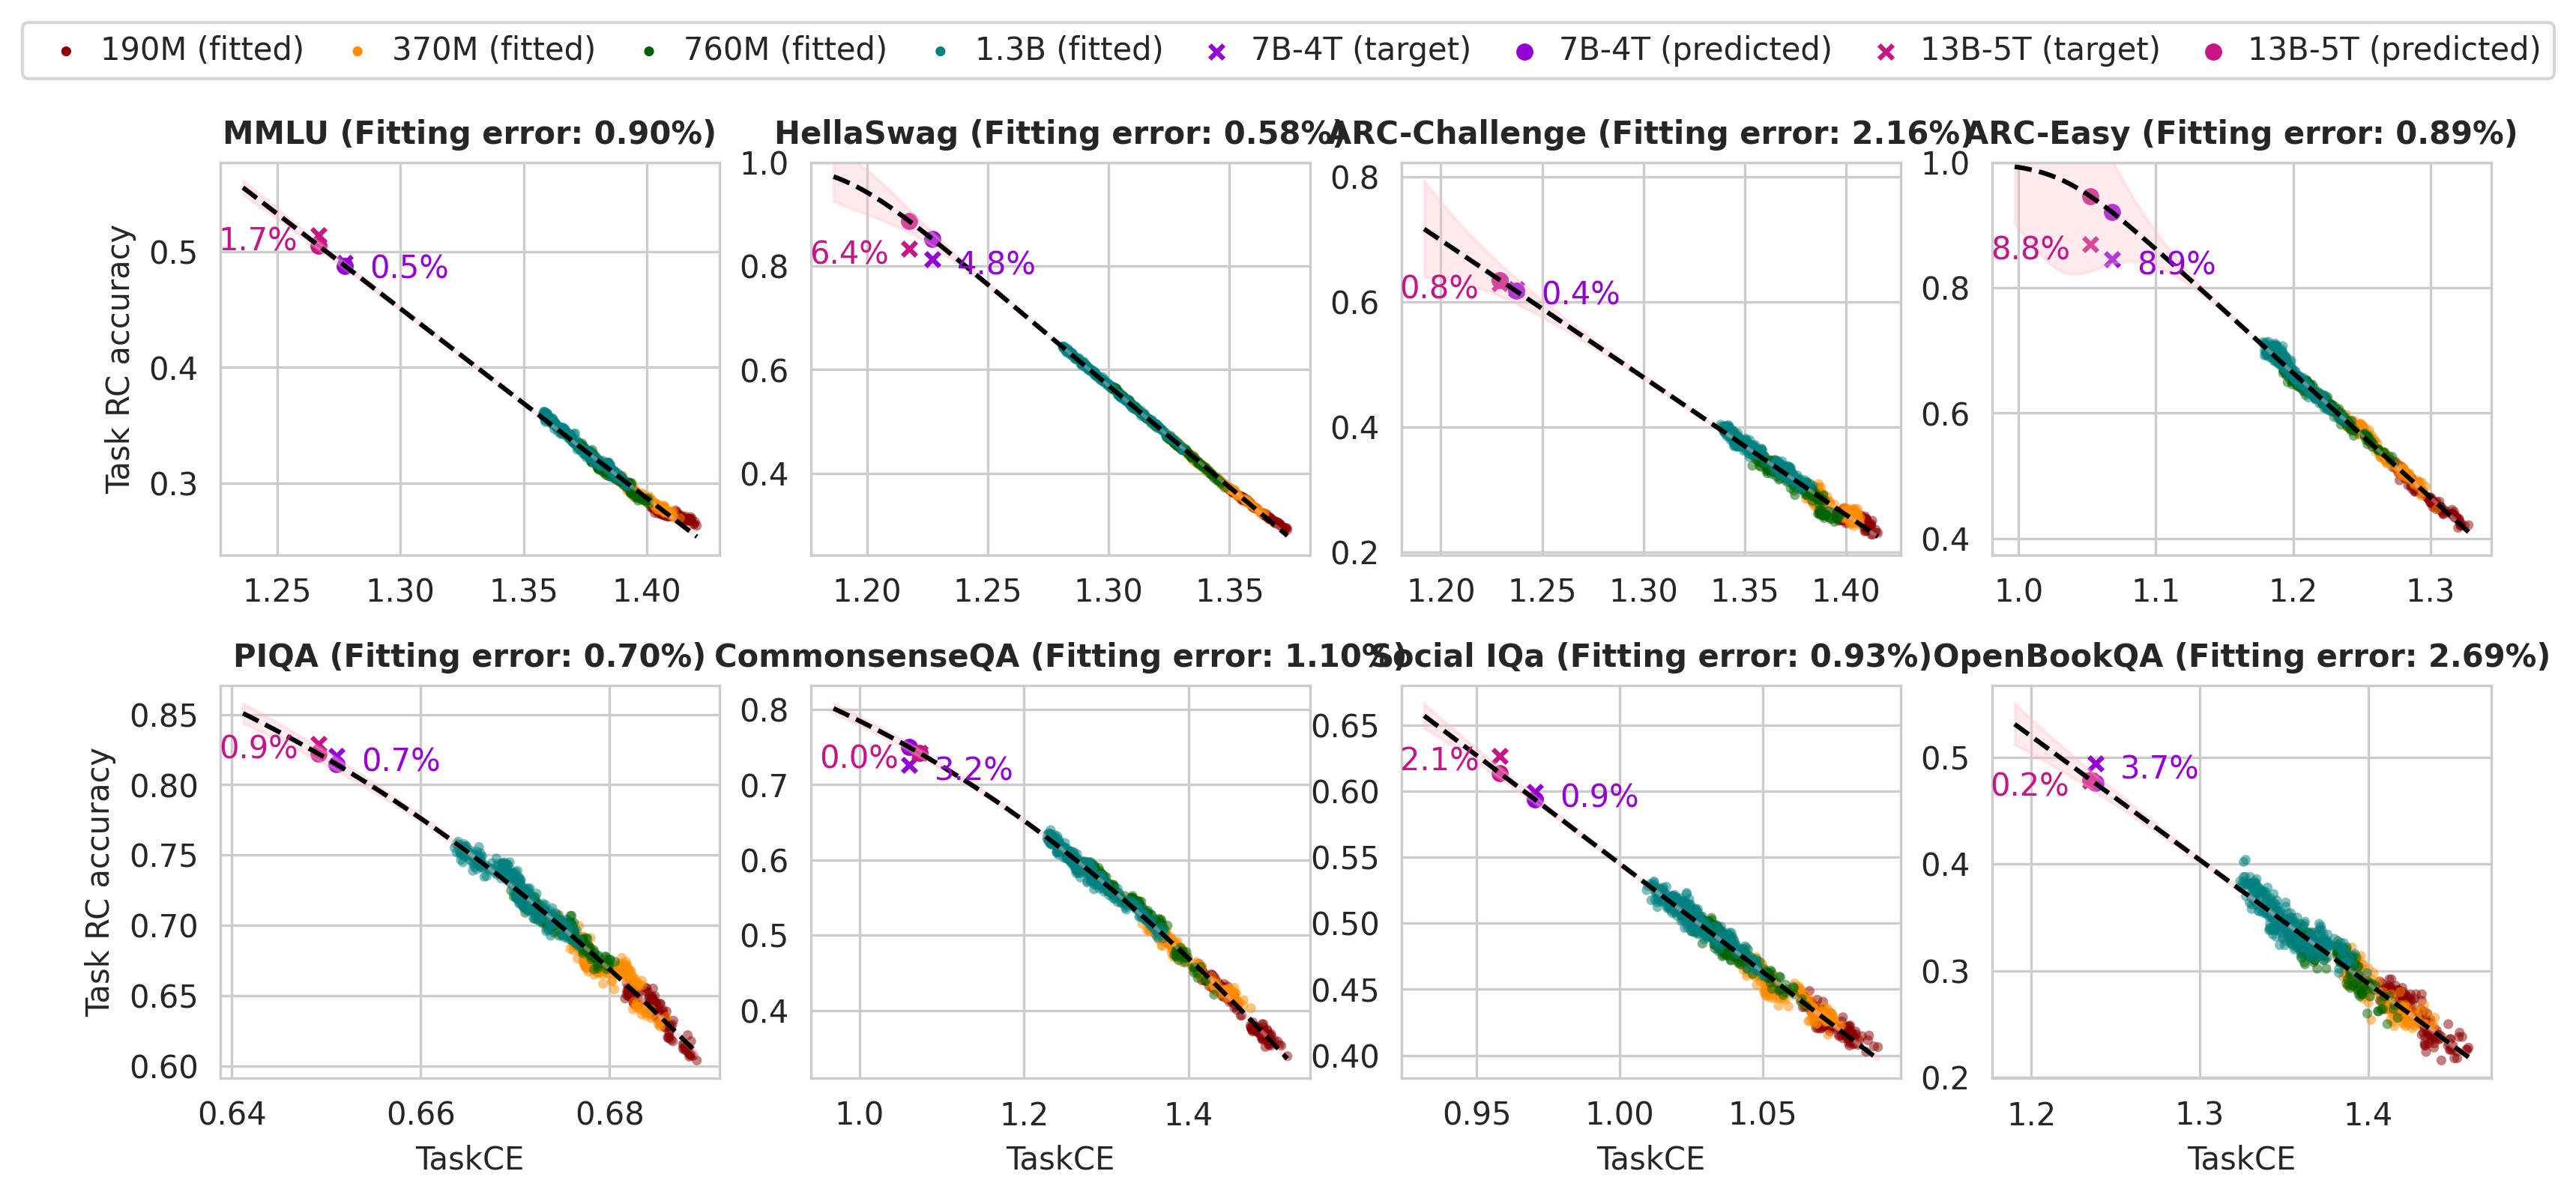
\includegraphics[width=\linewidth]{images/step2_taskce_main.png}
    \caption{Predicting the task metric from the \textit{task cross-entropy} (\autoref{eqn:task_ce}) in step 2.}
    \label{fig:step2_taskce}
\end{figure*}


\begin{figure*}[ht]
    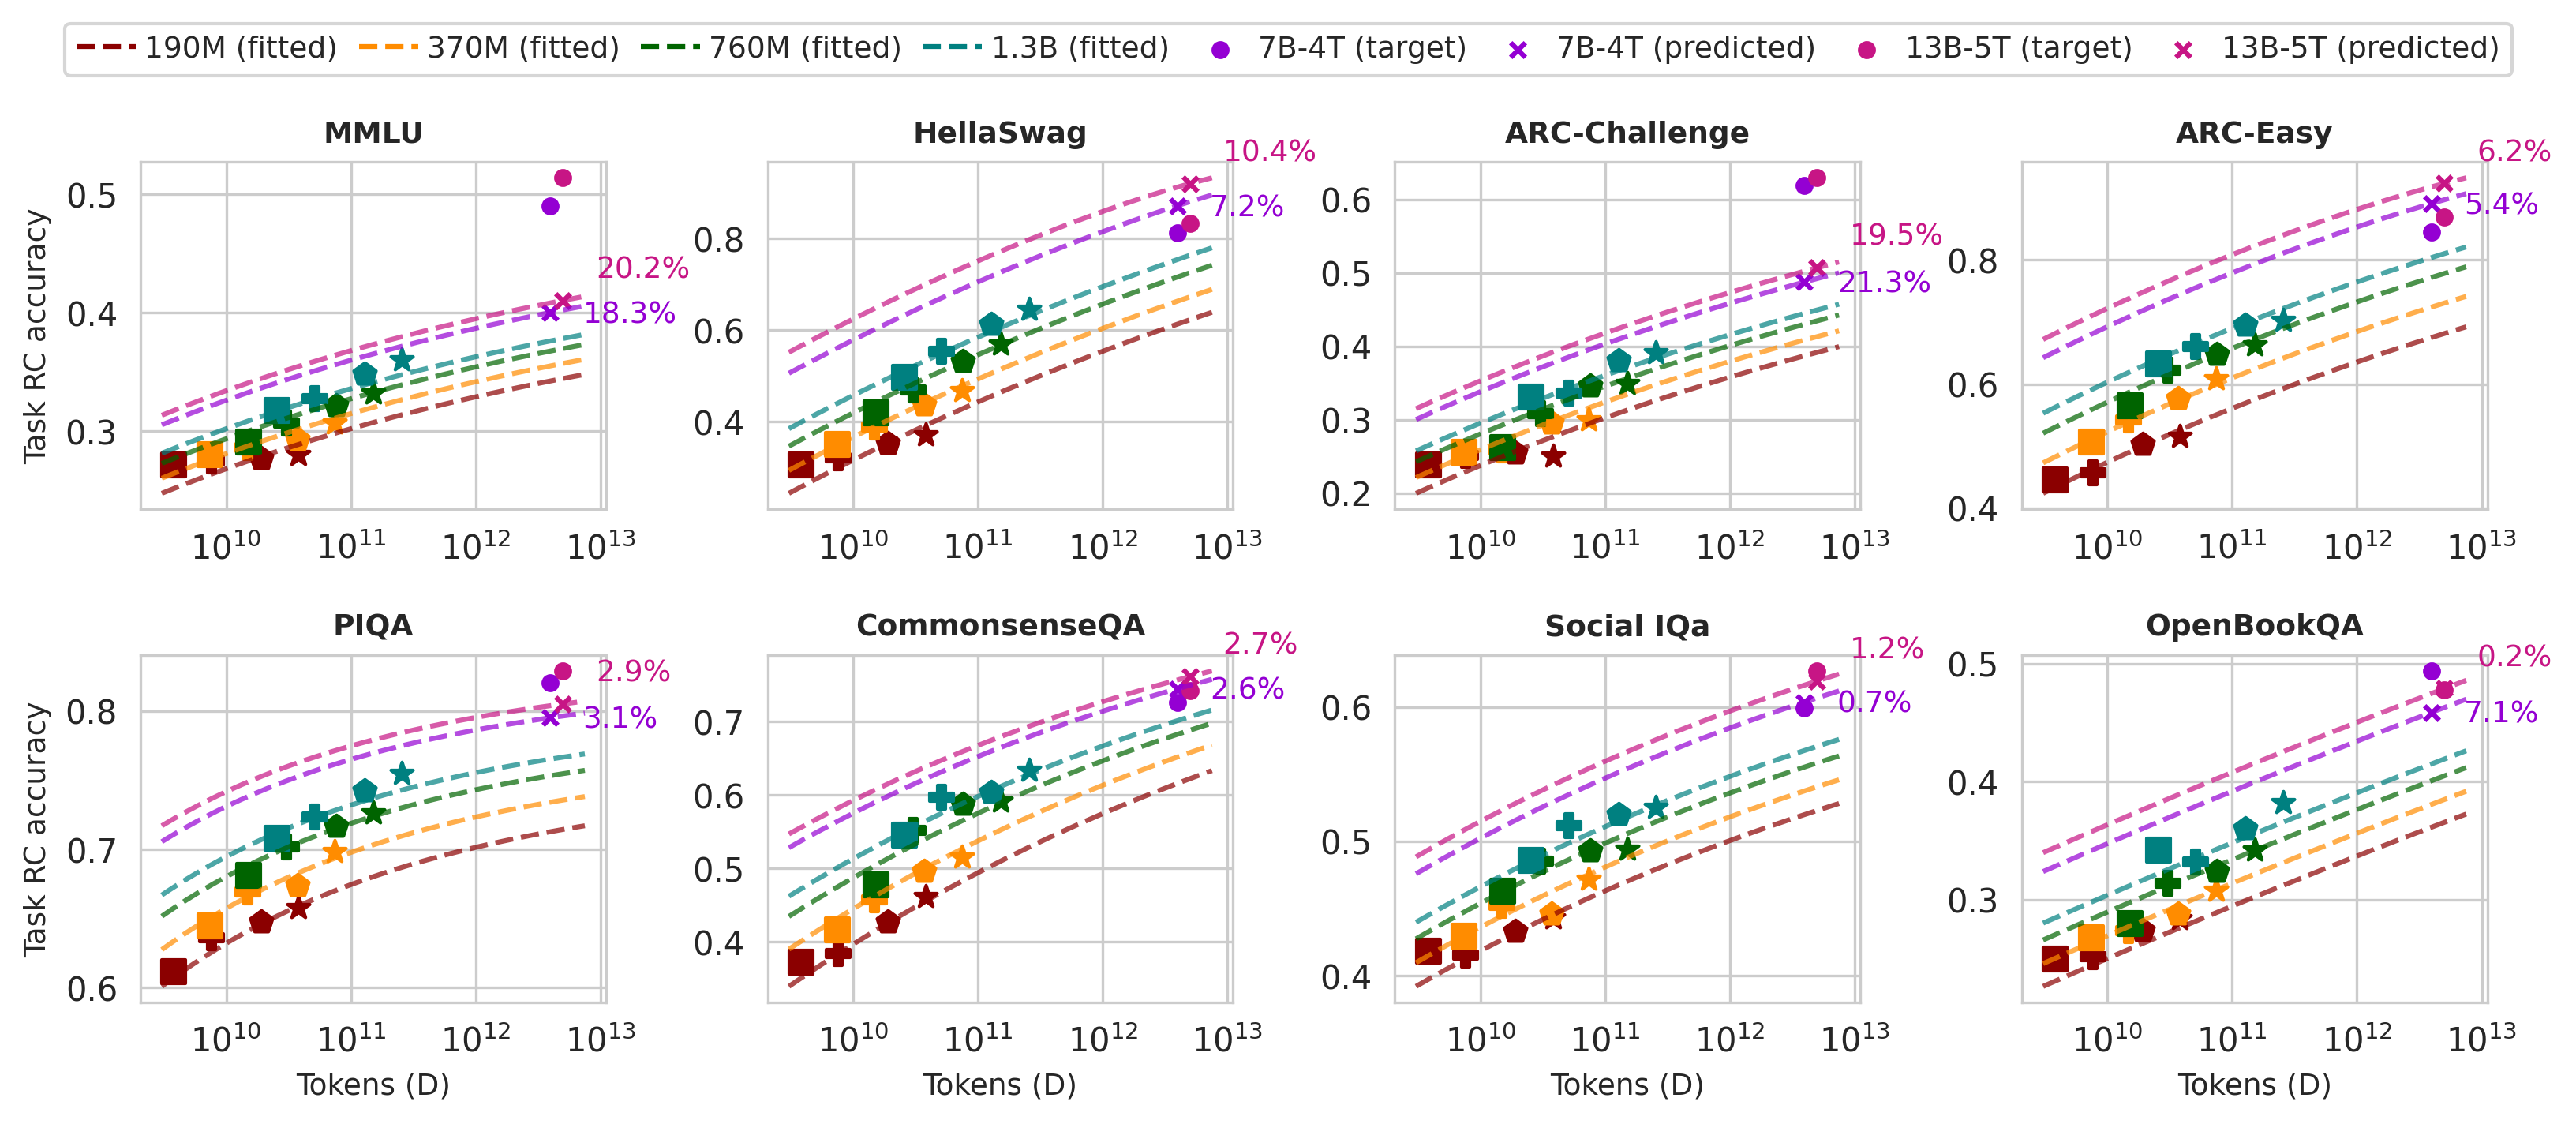
\includegraphics[width=\linewidth]{images/chained_taskce_main.png}
    \caption{Chaining predictions from step 1 (\autoref{fig:step1_taskce}) and step 2 (\autoref{fig:step2_taskce}) with \textit{task cross-entropy} as the intermediate feature.}
    \label{fig:chained_taskce}
\end{figure*}

% Our intermediate feature in step 1 is the conditional loss of the \textit{correct answer} of a task, from which we predict the accuracy in step 2. However, the accuracy is computed from the losses of both correct and incorrect continuations, as seen in \autoref{eqn:task_acc}.

\paragraph{Step 2 scaling with Task Cross-Entropy.} When inspecting the ladder models, we notice that the task cross-entropy correlates with accuracy in a more linear fashion than is the case for BPB.
We therefore seek for a function $Acc(TaskCE)$ that is linear for large values of $TaskCE$, but for small values of $TaskCE$ should approach an asymptote of perfect accuracy (where all the probability mass is concentrated on the correct answer). 
A good candidate for this transition is the log-sigmoid function, leading us to conjecture the following formula:

\begin{equation} \label{eqn:log_sigmoid}
Acc(TaskCE) = 1 - a\log \sigma\left(-k (TaskCE - TaskCE_0)\right),
\end{equation}

where $\sigma(\cdot)$ is the sigmoid function, and $a, k, TaskCE_0$ are constants to be fit.
This expression is not valid in the regime of large task cross-entropies, where models perform random guessing. Thus, we only use data points from the last 50\% of training for curve fitting.



\paragraph{Results.} \autoref{fig:step1_taskce} and \autoref{fig:step2_taskce} show the results of fitting step 1 and step 2 with the task cross-entropy as output and input variable, respectively. 
\autoref{fig:chained_taskce} visualizes the predictions of combining these two steps, and  \autoref{tab:updated_pred_taskce} compares the predictions errors between using task cross-entropy or the correct answer loss as the intermediate feature. We make the following observations:
\begin{itemize}[leftmargin=16pt]
\item In step 2, the task cross-entropy is overall a more accurate predictor of RC accuracy: The average prediction errors across 7B and 13B models is 2.75\% vs. 3.6\% for the correct answer loss in \autoref{fig:step2}. 
We note that the step 2 fit in \autoref{fig:step2_taskce} is particularly good on ARC-Challenge and OpenBookQA, but substantially worse on HellaSwag. We note all our observations for HellaSwag are in the ``linear'' regime of the log-sigmoid, making it difficult to estimate the curvature of the transition to the horizontal asymptote.

\item The average fitting and extrapolation errors in step 1 of \autoref{fig:step1_taskce} are moderate and comparable to \autoref{fig:step1}. However, we notice that the fitting errors for TaskCE tend to be more skewed, i.e., the fitted Chinchilla curves tend to underestimate the performance of the 190M-1xC model and overstimate the 190M-10xC, while underestimating the 1B-1xC and overestimating the 1B-10xC. As these errors appear more systematic, it raises questions whether this parametric form is a good fit over much larger scales. Notably, it results in substantial errors in the task cross-entropy of MMLU and ARC-Challenge (4.2\% - 4.8\%).

\item Finally, we note that the values for TaskCE fall into a narrow range. This means that the predictions in step 2 are highly sensitive to small changes in the task cross-entropy, e.g., a difference in task cross-entropy of less than $0.05$ nats in PIQA can make the difference between random task accuracy (at $TaskCE = 0.69$) and 83\% accuracy (at $TaskCE = 0.65$). As a consequence, small relative errors in step 1 (0.6\% for the 13B model on PIQA) are amplified in Step 2 and result in larger overall errors in accuracy (2.9\% for PIQA), despite a good fit in step 2 (0.9\% prediction error for the 13B accuracy). Similarly, a step-1 prediction error of 4.7\% for the 13B model on ARC-Challenge results in an overall error of 19.5\%.
\end{itemize}

\subsection{General language modeling loss as the intermediate feature}
\label{app:c4}

Language modeling loss (LM loss) on held-out sets has been shown to follow the power law \citep{Hoffmann2022TrainingCL}.
Here, we consider if we can map it to task performance.

We experiment with using the LM loss on the C4-en validation set \citep{Raffel2019ExploringTL} as the intermediate feature.

\begin{figure*}[t]
\small
\setlength{\tabcolsep}{3pt}
\centering
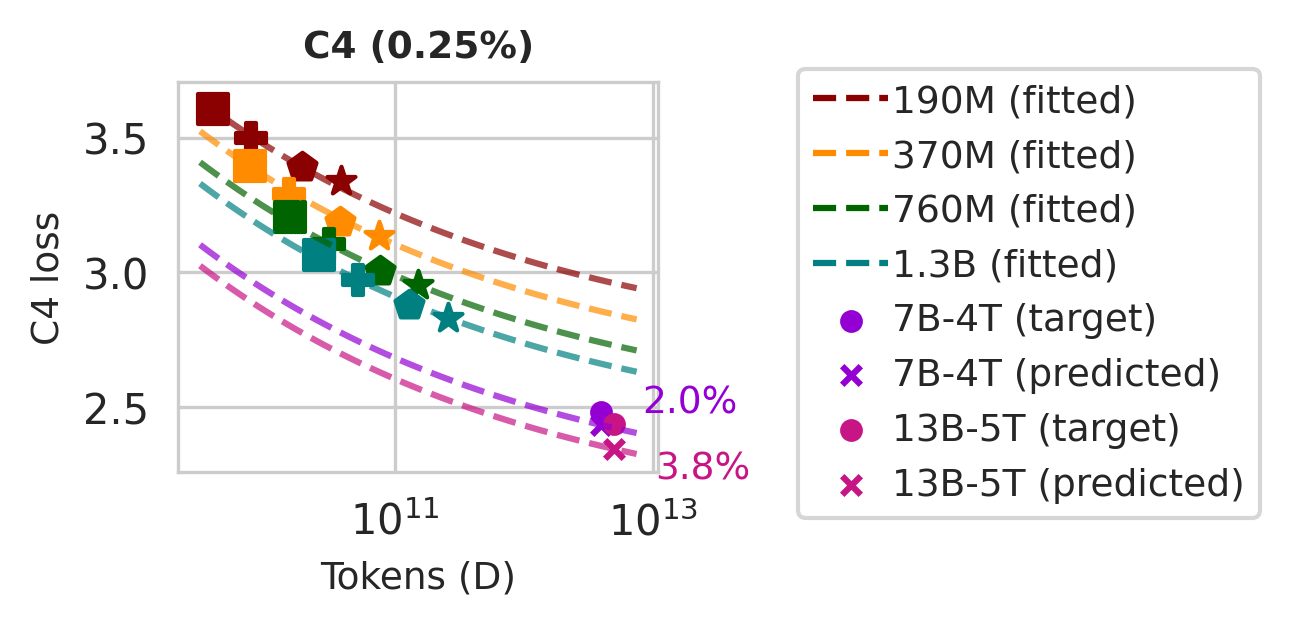
\includegraphics[width=0.5 \linewidth]{images/step1_c4_main.png}
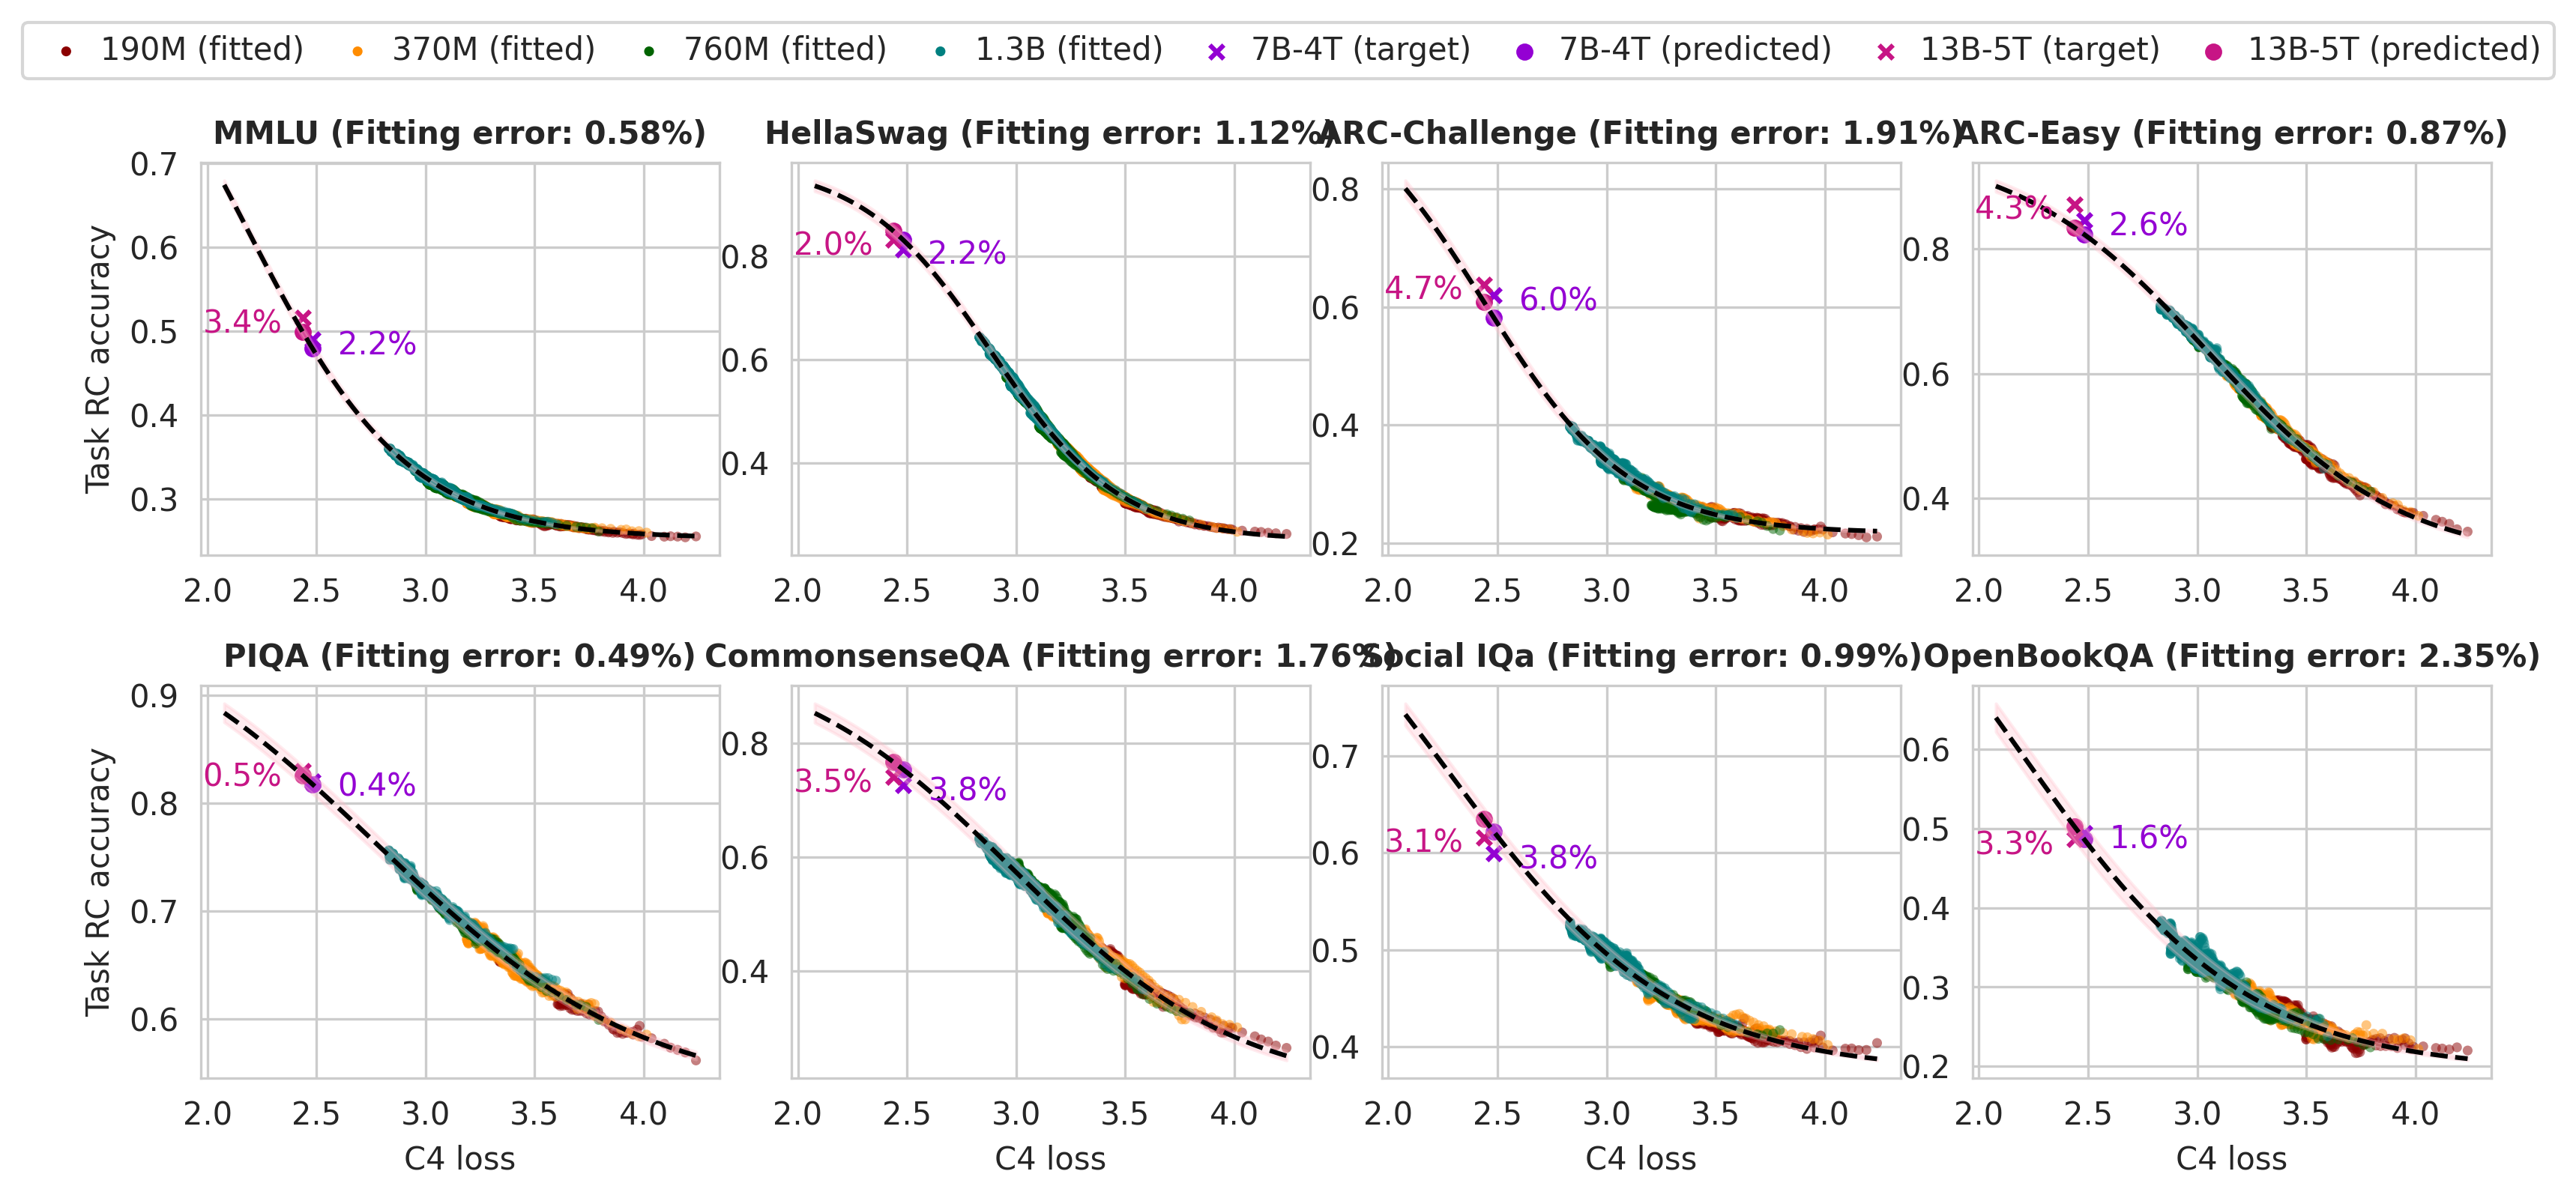
\includegraphics[width=\linewidth]{images/step2_c4_main.png}
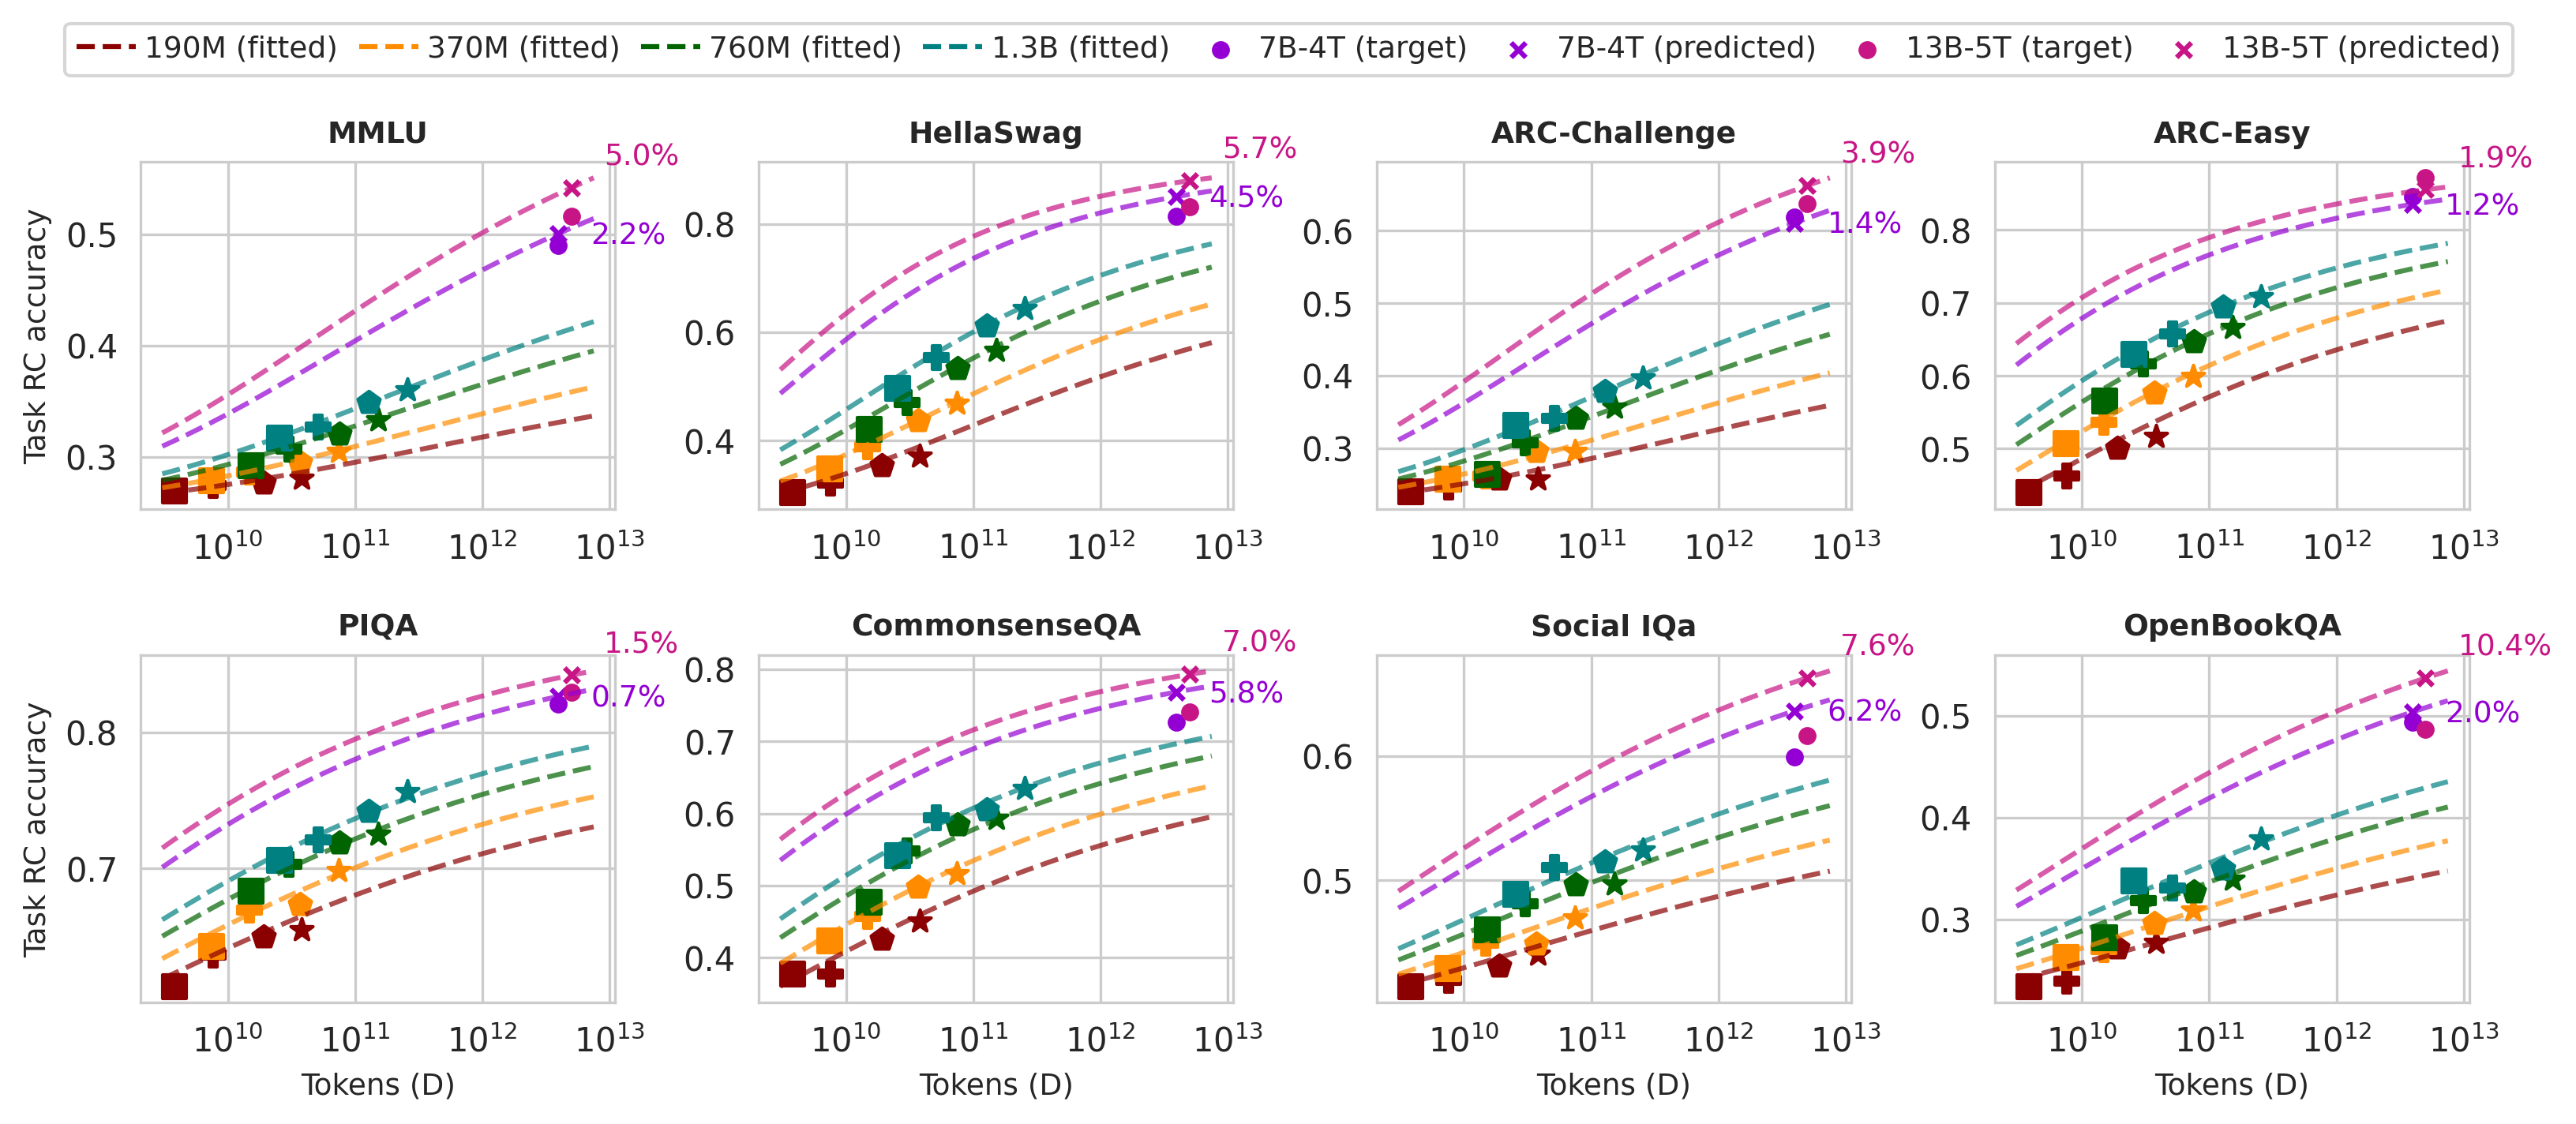
\includegraphics[width=\linewidth]{images/chained_c4_main.png}
% \begin{tabular}{c l | r r r r | r r r r}
% \toprule
% & & \multicolumn{4}{c|}{\textbf{7B-4T}} & \multicolumn{4}{c}{\textbf{13B-5T}} \\
% & & Pred & Actual & Error & \%Error & Pred & Actual & Error & \%Error \\
% \midrule
% \multirow{8}{*}{\textbf{RC}} & MMLU & 50.1 & 49.0 & 1.1 & 2.2\% & 54.2 & 51.6 & 2.6 & 5.0\% \\
% & HellaSwag & 85.0 & 81.3 & 3.7 & 4.5\% & 87.9 & 83.2 & 4.7 & 5.7\% \\
% & ARC-Challenge & 61.1 & 61.9 & 0.8 & 1.4\% & 66.3 & 63.8 & 2.5 & 3.9\% \\
% & ARC-Easy & 83.5 & 84.6 & 1.1 & 1.2\% & 85.5 & 87.2 & 1.7 & 1.9\% \\
% & PIQA & 82.6 & 82.0 & 0.6 & 0.7\% & 84.2 & 83.0 & 1.2 & 1.5\% \\
% & CommonsenseQA & 76.8 & 72.6 & 4.2 & 5.8\% & 79.3 & 74.1 & 5.2 & 7.0\% \\
% & Social IQa & 63.6 & 59.9 & 3.7 & 6.2\% & 66.3 & 61.6 & 4.7 & 7.6\% \\
% & OpenBookQA & 50.4 & 49.4 & 1.0 & 2.0\% & 53.7 & 48.6 & 5.1 & 10.4\% \\
% \bottomrule
% \end{tabular}
\caption{
    Using language modeling loss on C4-en validation as the intermediate feature.
    \textbf{From top to bottom}: step 1, step 2, and chaining the two steps.
}
\label{fig:c4}
% \vspace{-16pt}
\end{figure*}

\autoref{fig:c4} shows the function fitting and predictions.

In step 1, the fitted function underestimates the C4 loss by 2.0\% for 7B-4T and 3.8\% for 13B-5T.
This error is higher than that on task loss prediction for 4 out of 8 tasks.
The step 2 error is also higher than using task loss on 4 out of 8 tasks.
When chaining the two steps to predict task accuracy, using C4 loss as intermediate feature resulted in higher error on 5 tasks -- MMLU, HellaSwag, CommonsenseQA, Social IQA, and OpenBookQA.
Prediction error is lower on ARC-Challenge and ARC-Easy.
We conclude that using C4 loss can benefit certain tasks where task loss does not work well. %\footnote{We use task loss in our main method because of its superiority on predicting MMLU.}.

\subsection{Comparison of three intermediate features}

\begin{figure*}[!h]
\centering
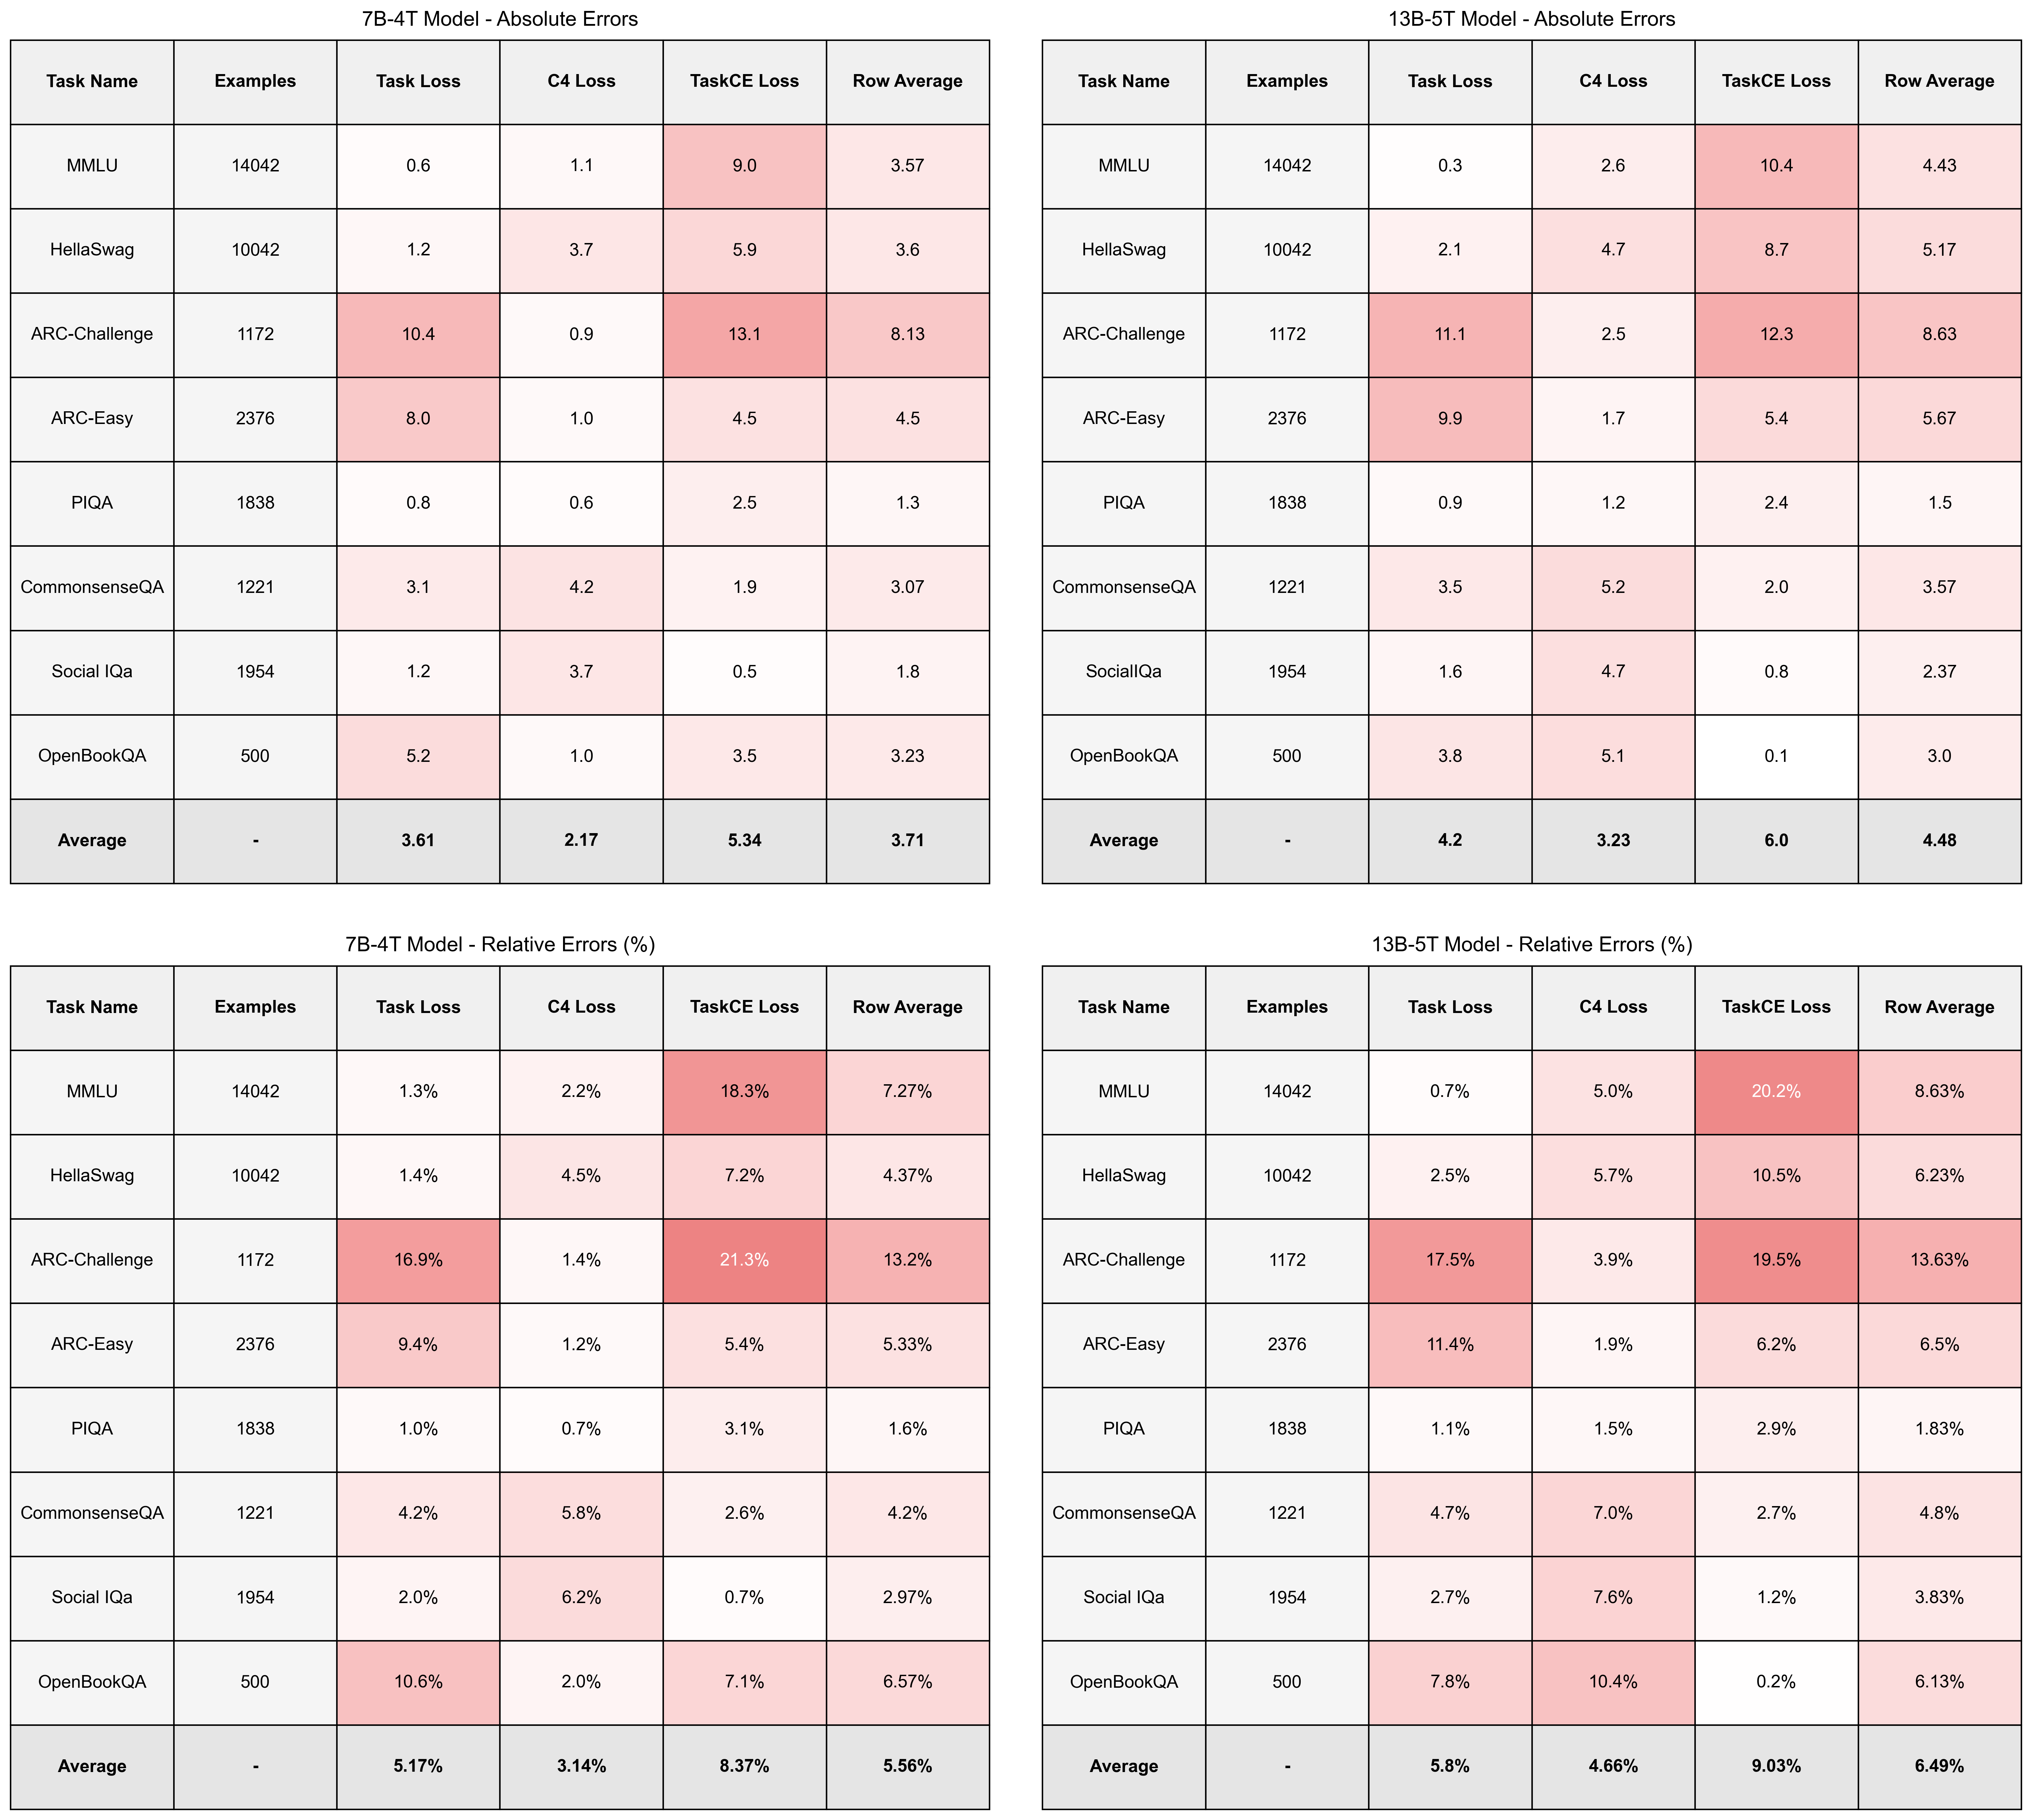
\includegraphics[width=0.99\linewidth]{images/intermediate_feature_comparison.png}
\vspace{-12pt}
\caption{
    Comparison of absolute and relative prediction errors for all three intermediate features. Using C4 as the intermediate works well for certain tasks, but results in overall higher errors. Task loss and TaskCE loss perform comparably. However, MMLU and HellaSwag have higher number of instances, and task loss performs better for them.
}
\label{fig:intermediate_feature_comparison}
\vspace{-8pt}
\end{figure*}

\subsection{Combining step 1 and 2 into a single step}
\label{app:single_step}

Here, we try to directly predict task accuracy from the training scale $(N, D)$ in one step, by combining \autoref{eqn:power} and \autoref{eqn:sigmoid} into a single parameterized function, and merging parameters $k$ and $L_0$ into $A, B, E$, so that we reduce to 7 free parameters:
% \begin{align*}
% Acc(N, D) = \frac{a}{1 + \exp \big( -k (A / N^\alpha + B / D^\beta + E - L_0) \big)} + b
% \end{align*}
% and we merge parameters $k$ and $L_0$ into $A, B, E$, so that we reduce to 7 free parameters:
\begin{align}
Acc(N, D) = \frac{a}{1 + \exp \big( -(A / N^\alpha + B / D^\beta + E) \big)} + b
\label{eqn:single_step}
\end{align}

With this, we remove the \textit{a priori} definition of a specific intermediate feature (i.e., the $A / N^\alpha + D / D^\beta + E$ expression no longer carries a specific meaning), while preserving the representation power of the function.
This function can be harder to fit, since it has more free parameters, is not convex, and we cannot use any data points collected from intermediate checkpoints as we did in step 2.

We fit this function with data points from the final checkpoints of the ladder models, using the same optimization method as in step 1 (\autoref{fig:single_step}). 
The prediction error is higher on 4 out of 8 tasks -- MMLU, ARC-Challenge, CommonsenseQA, and Social IQA.
In particular, on CommonsenseQA the fitted functions does not vary with respect to model size, indicating a degenerated function fitting.
We conclude that the single-step approach is not as robust as the two-step approach.

\begin{figure*}[t]
\centering
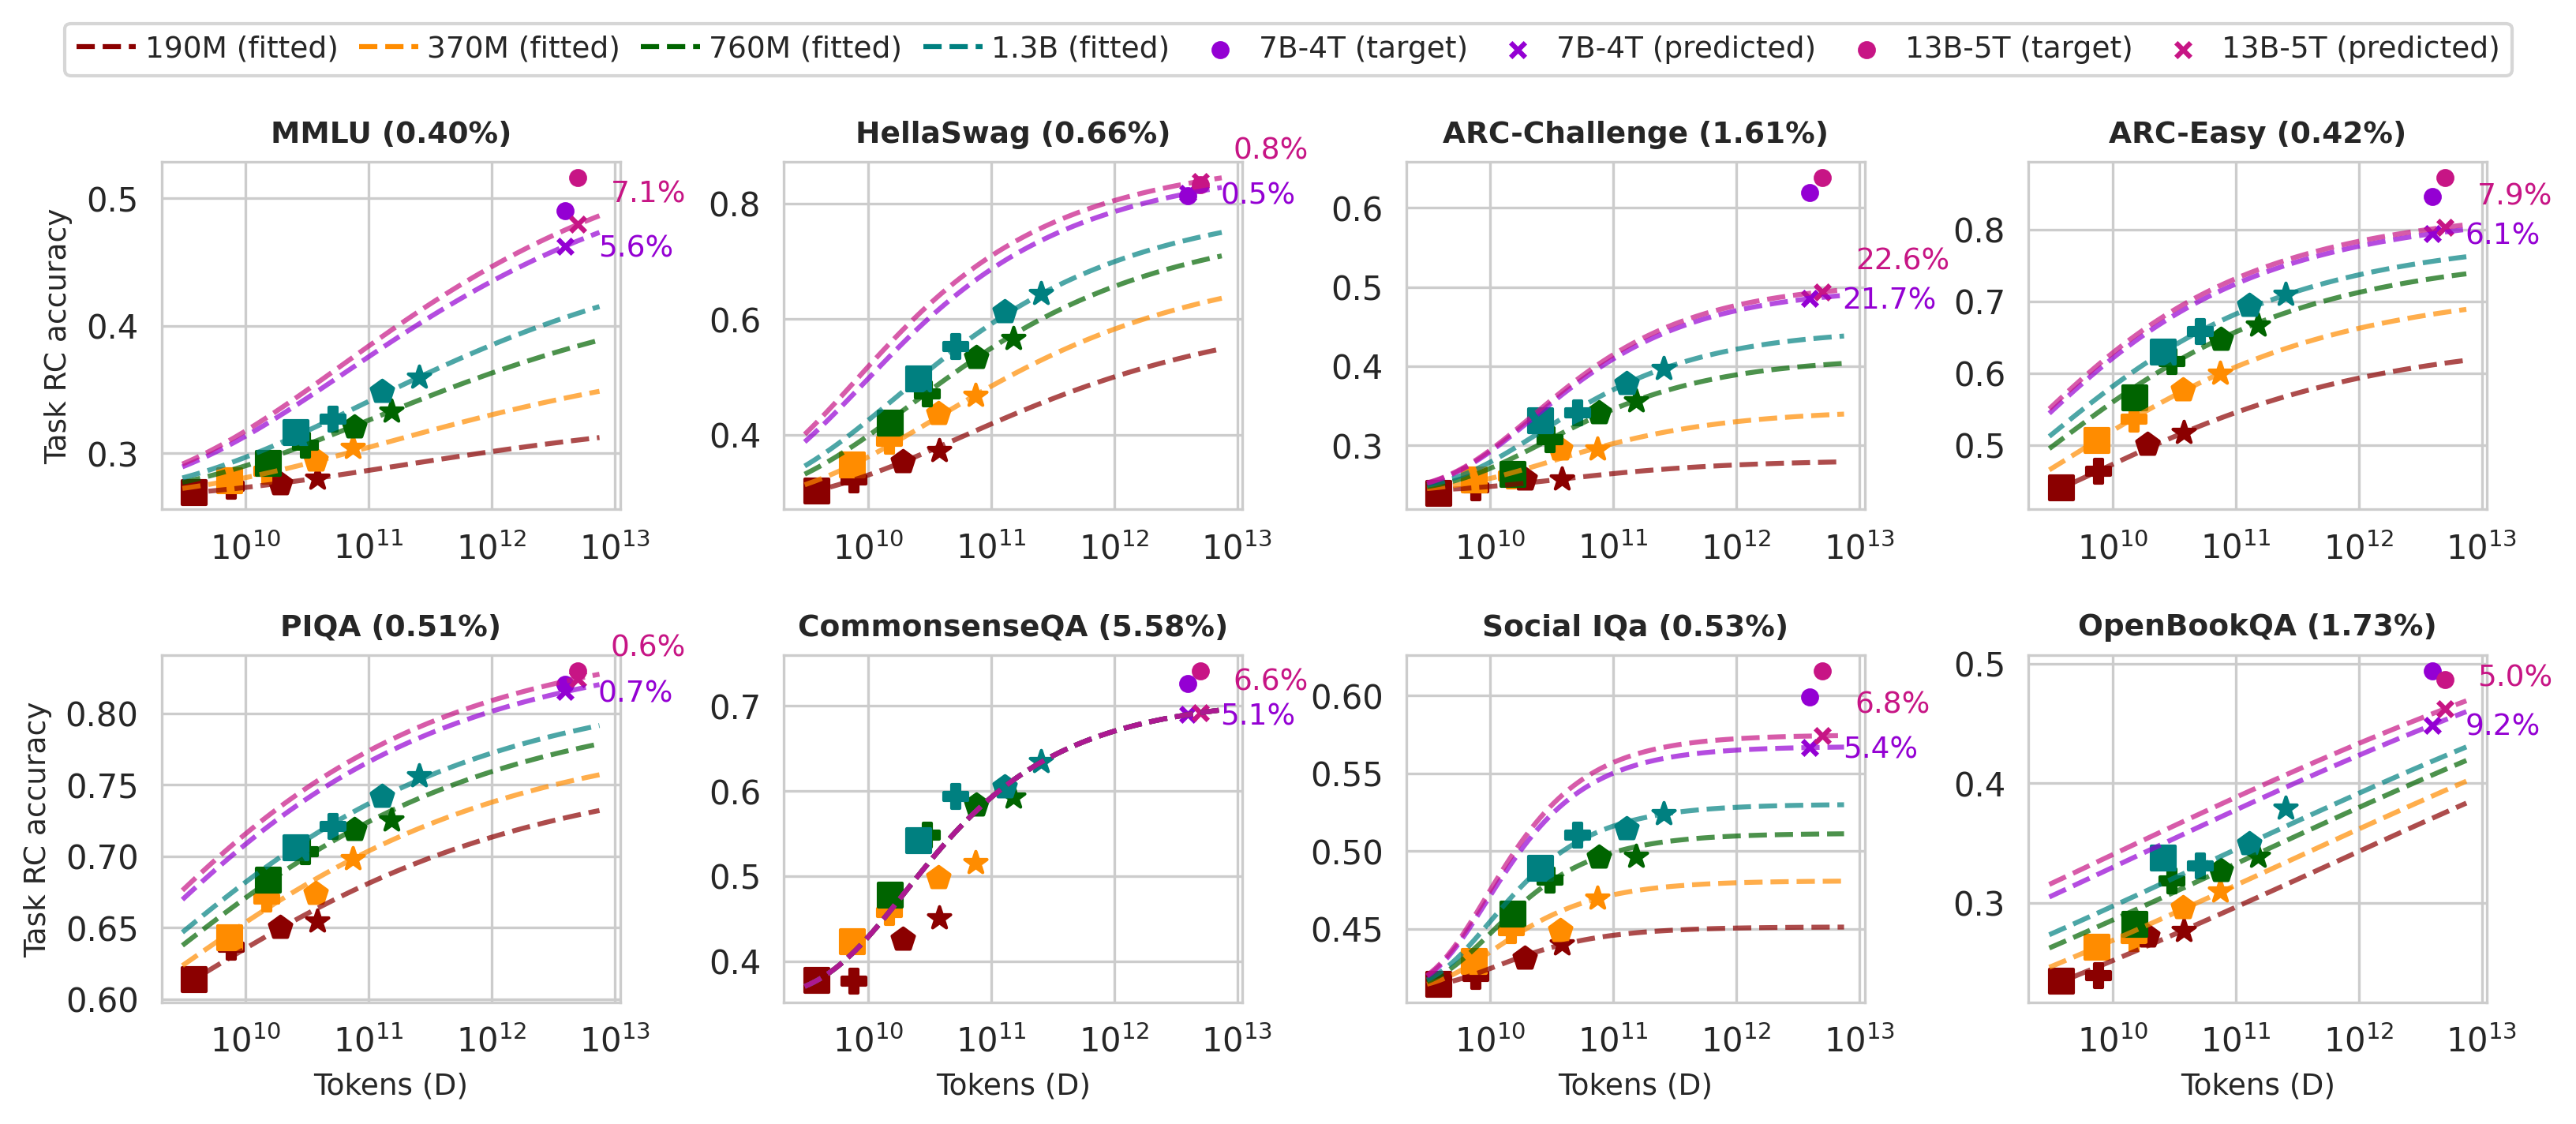
\includegraphics[width=\linewidth]{images/single_step_main.png}
\caption{
    Task RC accuracy vs training scale $(N, D)$, with fitting on the single-step function in \autoref{eqn:single_step}.
}
\label{fig:single_step}
% \vspace{-16pt}
\end{figure*}

\section{Scaling law predictions for 32B-6T}
\label{app:32B-6T}

We demonstrated our method on 7B-4T and 13B-5T models, using only 1\% of the compute required for the target models. Here, we test the robustness of the ladder, by trying to predict the accuracies for a much larger model of the same family: \basemodelname{} 32B, trained to 6T tokens (32B-6T). This model was trained with $1.15 \times 10^{24}$ FLOPs, and the ladder models account for only 0.45\% of the compute of this model. 

\begin{figure*}[t]
\small
\setlength{\tabcolsep}{3pt}
\centering
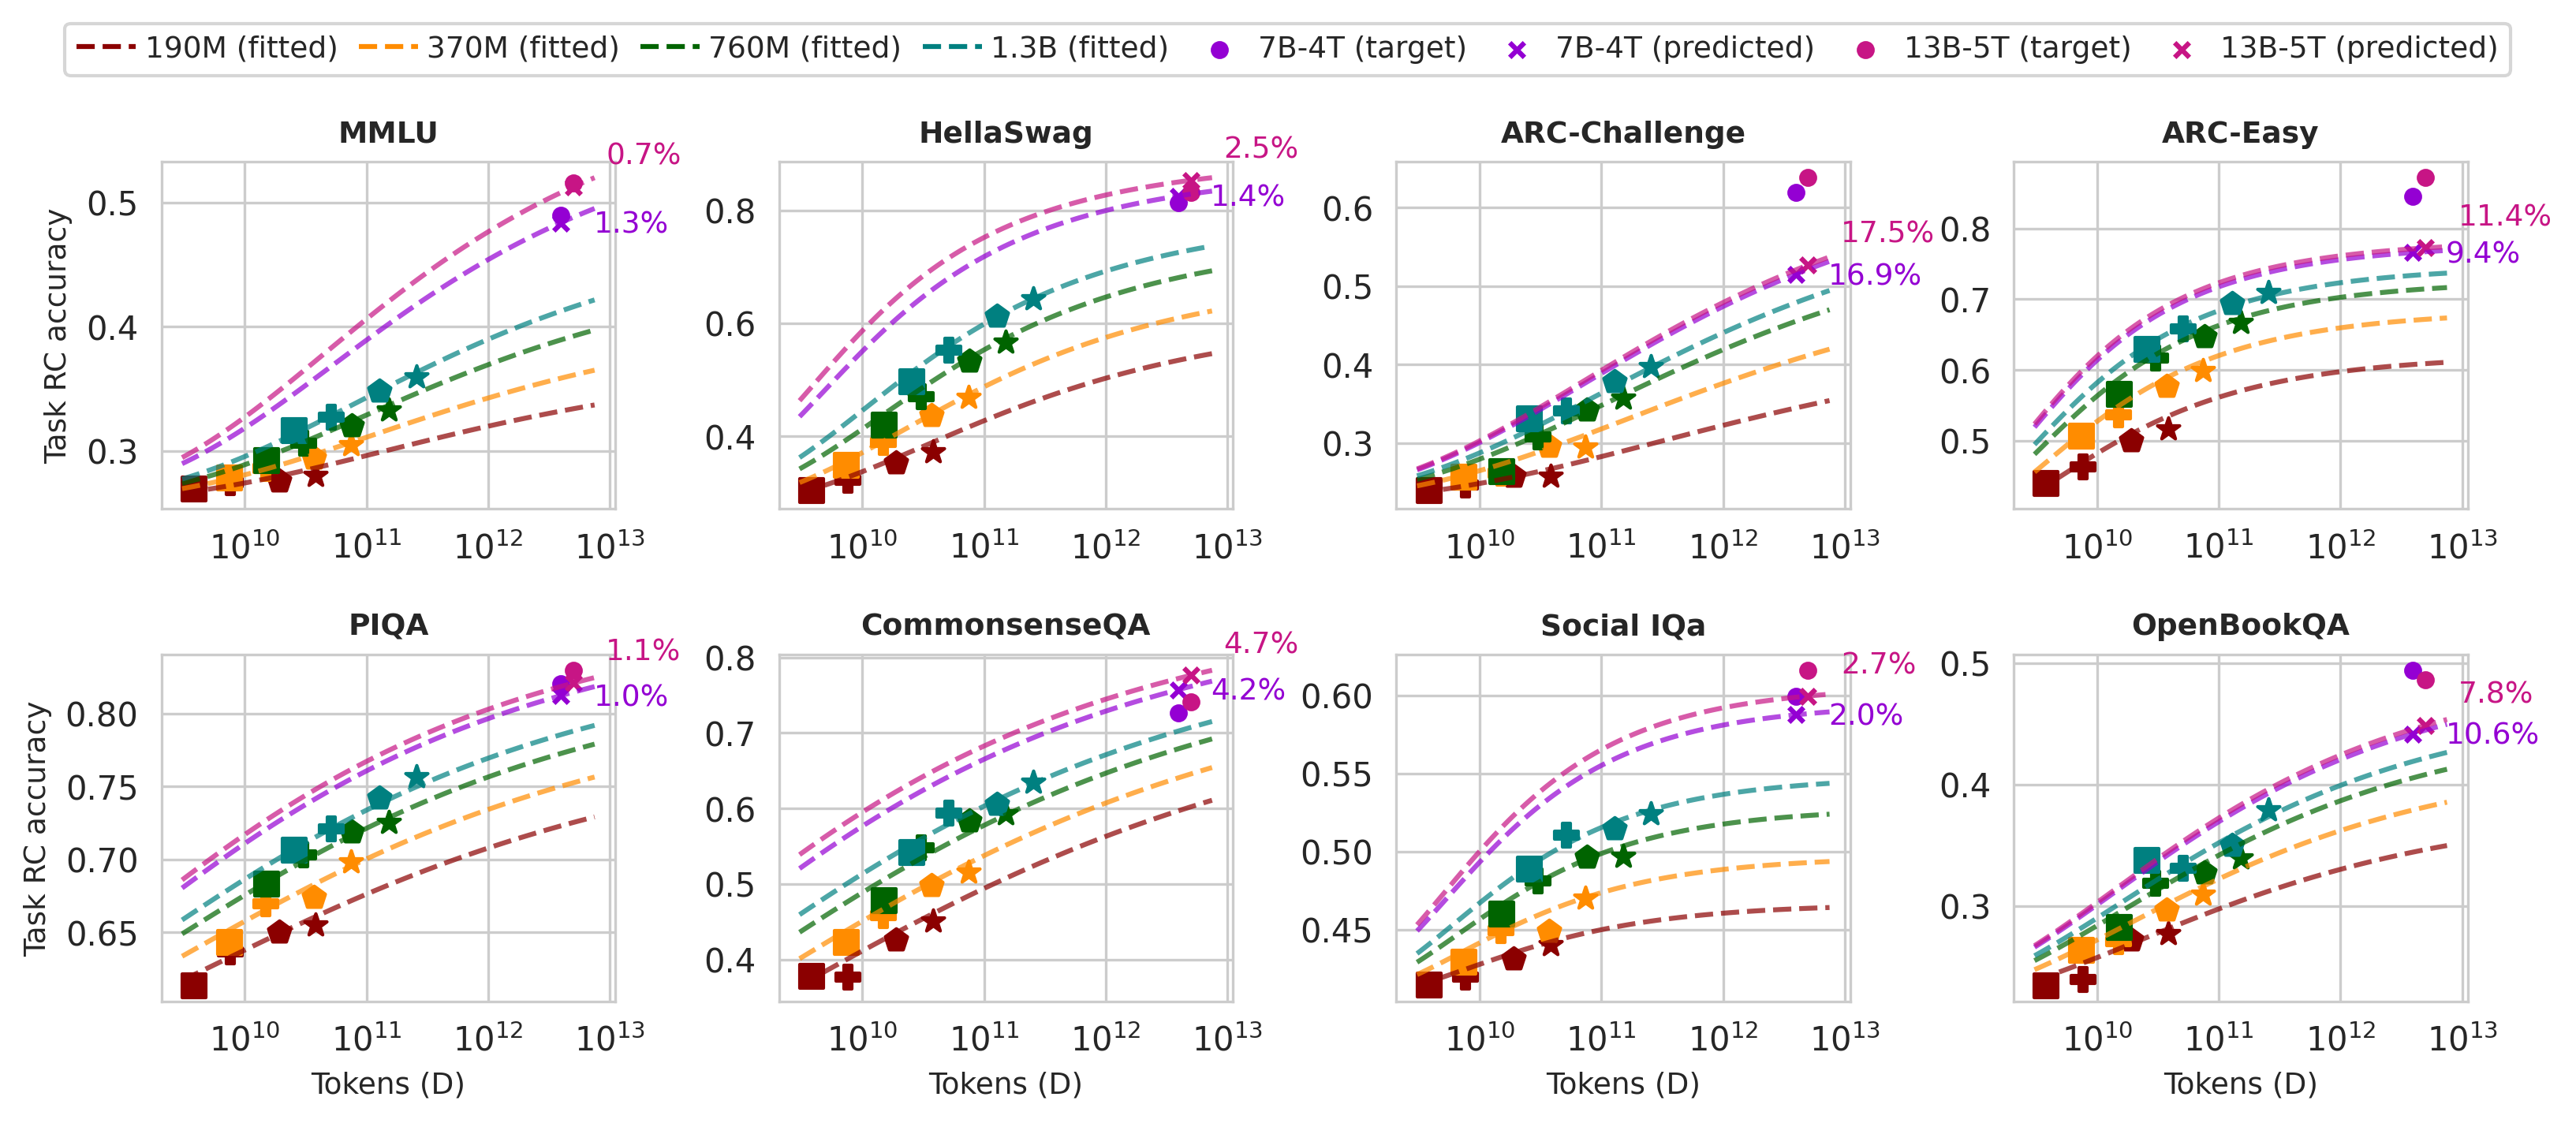
\includegraphics[scale=0.5]{images/chained_main.png}
\resizebox{0.75 \textwidth}{!}{%
\begin{tabular}{l | r r r r}
\toprule
& \multicolumn{4}{c}{\textbf{32B-6T}} \\
\textbf{Task} & Pred & Actual & Error & \%Error \\
\midrule
%MMLU & 48.4 & 49.0 & 0.6 & 1.3\%  \\
HellaSwag & 88.0 & 85.3 & 2.7 & 3.07\% \\
ARC-Challenge & 53.6 & 66.8 & 13.2 & 24.63\% \\
ARC-Easy & 77.8 & 88.8 & 11.0 & 14.14\% \\
PIQA & 82.9 & 83.6 & 0.7 & 0.84\% \\
CommonsenseQA & 79.5 & 75.4 & 4.1 & 5.16\% \\
Social IQa & 61.1 & 62.3 & 1.2 & 1.96\% \\
OpenBookQA & 45.4 & 53.2 & 7.8 & 17.18\% \\
\midrule
Average & -- & -- & 5.81 & 9.57\% \\
\bottomrule
\end{tabular}
}%
\caption{
Task accuracy prediction for the 32B model using task loss as the intermediate feature.
\ding{110} = 1xC; \ding{58} = 2xC; $\pentagofill$ = 5xC; $\bigstar$ = 10xC.
Prediction error is next to the target.}
\label{tab:stacked_preds_32b}
\vspace{-8pt}
\end{figure*}

% Task	Pred	Actual
% HellaSwag	88.0	85.3
% ARC-Challenge	53.6	66.8
% ARC-Easy	77.8	88.8
% PIQA	82.9	83.6
% CSQA	79.5	75.4
% Social IQA	61.1	62.3
% OpenBookQA	45.4	53.2

\autoref{tab:stacked_preds_32b} shows the predictions and errors for 32B-6T model. As expected, and following from \ref{app:ablate_compute}, the overall prediction error is higher %\footnote{We do not report MMLU predictions as MMLU-RC is over-saturated for 32B.}.
We also observe a similar trend of higher errors for high variance tasks like ARC-C and ARC-E as with the smaller target models.
However, for lower-variance tasks such as HellaSwag, PiQA, and SocialIQA, we can still predict the accuracy within an absolute error of 3 points.  This indicates that the ladder models are fairly robust in their prediction abilities even as the target model is scaled to be much larger.